% Copyright (C)  2010-2013  W.Trevor King <wking@tremily.us>
% Permission is granted to copy, distribute, and/or modify this document
% under the terms of the Creative Commons Attribution-ShareAlike License
% Version 3.0.
% 
% You should have revieved a copy of the Creative Commons
% Attribution-ShareAlike License along with this program (COPYING-CC);
% if not, visit
%   http://creativecommons.org/licenses/by-sa/3.0/legalcode

\documentclass[%
  subfig,%
  indenttoc,%
  approvalform,%
  final%
%  draft%
]{drexel-thesis}
% See drexel-thesis.pdf for more options.

%\includeonly{%
%  cantilever/main,%
%  temperature/main%
%  cantilever-calib/main
%}

\author{William Trevor King}
\title{Open source single molecule force spectroscopy}
\DUTmonth{June}
\DUTyear{2013}
\degree{Doctor of Philosophy}
\advisor{Guoliang Yang, Ph.D.}
\advisor{Luis Cruz Cruz, Ph.D.}
\copyrighttext{\copyrighttextCCBYSA}

% Remove the \leftmark (chapter title), since some chapter/section
% titles would overlap.
\fancyfoot[RE,LO]{}

%\usepackage[utf8]{inputenc} % Allow UTF-8 characters in input files

\usepackage[super,sort&compress,comma]{natbib} % fancy citation extensions
% super selects citations in superscript mode
% sort&compress automatically sorts and compresses compound citations (\citep{a,b,...})
% comma seperates multiple citations with commas rather than the default semicolons.

\bibliographystyle{unsrtnat} % Number citations in the order referenced.

% use symbols for footnotes, so they aren't confused with references
%\usepackage[symbol*]{footmisc}

% Formatting stuff for the curriculum vitae
\usepackage{bibunits}
\defaultbibliography{blurb/main,root}
\defaultbibliographystyle{plain}
\usepackage[ManyBibs,LabelsAligned]{currvita}

% Nicer references with \cref, \Cref, etc.
\usepackage[capitalize]{cleveref}

% For defining my own \fref command
\usepackage{boolexpr}
\usepackage{pdftexcmds}

% Epigraphs (chapter-leading quotations)
\usepackage{epigraph}
\setlength{\epigraphwidth}{5in}

\usepackage{makeidx} % Indexing
\makeindex
\usepackage[intoc,noprefix]{nomencl} % Abbreviation indexing
% Prefixes:
%   o :    Operators and function symbols
%   sg :   Greek symbols
%   so :   Other (non-Greek/Roman symbols)
%   sr :   Roman symbols
%   text : Abbreviations, chemical names, phrases, etc
\makenomenclature
\makeatletter
% override nomencl's thenomenclature to use drexel-thesis's listed@schapter
\def\thenomenclature{%
  \listed@schapter{\nomname}
  \nompreamble
  \list{}{%
    \labelwidth\nom@tempdim
    \leftmargin\labelwidth
    \advance\leftmargin\labelsep
    \itemsep\nomitemsep
    \let\makelabel\nomlabel}}
\makeatother
\iffinal{}{
  %\usepackage{showidx} % Print index keys in margins
  % for some reason, showidx disables Index generation...
  %\usepackage{showkeys} % Print labels in margins
}

% fix assorted LaTeX issues and defines \textsubscript
\usepackage{fixltx2e}
% environments for multiline displayed equations, and other enhancements
\usepackage{amsmath}
% proof environment and extensions for the \newtheorem command
\usepackage{amsthm}
%% The amssymb package provides various useful mathematical symbols
\usepackage{amssymb}
% fonts like mathbb (blackboard bold) and mathcal (caligraphic)
\usepackage{amsfonts}
% double struck math fonts
\usepackage{dsfont}
% nicer table formatting (\toprule, \cimidrule, \midrule, and \bottomrule)
\usepackage{booktabs}
% syntax highlighting for source code
\usepackage{minted}
% for table alignment on decimals (and maybe for units later)
\usepackage{siunitx}
% for \NewDocumentCommand
\usepackage{xparse}

\usepackage{xcolor}

% The lineno packages adds line numbers. Start line numbering with
% \begin{linenumbers}, end it with \end{linenumbers}. Or switch it on
% for the whole article with \linenumbers after \end{preamble}.
% Note that line numbering messes with TOC/LOT/LOF \numberline,
% so ensure line numbering is off for the tables.
\iffinal{}{\usepackage{lineno}}

\usepackage{pgf}          % fancy graphics
\usepackage{tikz}         % a nice, inline PGF frontend
\usetikzlibrary{automata} % graph-theory library
\usetikzlibrary{backgrounds} % background layers
\usetikzlibrary{calc}     % coordinate-calculation library
\usetikzlibrary{decorations.markings}       % custom marks
\usetikzlibrary{decorations.pathreplacing}  % braces and other fancy paths
\usetikzlibrary{topaths}      % 'curve to' style lines (in, out, etc.)
\usetikzlibrary{shapes.misc}  % for 'rounded rectangle'

\usepackage[inline]{asymptote}    % more fancy graphics ;).

\usepackage{epsdice}      % dice-face font

\usepackage{wtk_cmmds}    % common personal macros, in ~/texmf/tex/latex/
% String comparison for \fref
\makeatletter
\long\def\isequal#1#2{\pdf@strcmp{#1}{#2}}
\makeatother

% An reference index from an unspecified source
% usage: \iref{environment}{value}
% for example: \iref{equation}{75}
\newcommand{\iref}[2]{%
  \switch%
  \case{\isequal{#1}{equation}}%
    ({#2})%
  \otherwise%
    {#2}%
  \endswitch%
}

% A formatted reference from an unspecified source
% usage: \fref{environment}{value}
% for example: \fref{figure}{75}
\newcommand{\fref}[2]{%
  \switch%
  \case{\isequal{#1}{equation}}%
    Eq.~\iref{#1}{#2}%
  \case{\isequal{#1}{figure}}%
    Fig.~\iref{#1}{#2}%
  \case{\isequal{#1}{section}}%
    Section~\iref{#1}{#2}%
  \otherwise%
    \PackageError{fref}{
      \MessageBreak
      environment value >#2< unknown \MessageBreak
    }{possible values are: equation. \MessageBreak}%
  \endswitch%
}

% References to external figures, equations, etc.
% usage: \xref{key}{environment}{value}
% for example: \xref{roman12}{figure}{75}
\newcommand{\xref}[3]{\citet{#1} \fref{#2}{#3}}

% Fourier Transform to angular momentum space
\newcommand{\Four}[1]{\ensuremath{{\mathcal F}\left\{ {#1} \right\}}}
% Fourier Transform to frequency space
\newcommand{\Fourf}[1]{\ensuremath{{\mathcal F}_f\left\{ {#1} \right\}}}

% use e^{...} instead of exp ...
\renewcommand{\exp}[1]{\ensuremath{e^{#1}}}

% Symbol denoting the Langevin function
\newcommand{\Langevin}{\ensuremath{\mathcal{L}}}
% Symbol denoting big-O order of #1
\newcommand{\order}[1]{\ensuremath{\mathcal{O}\p({#1})}}

% Integral from #1 to #2 of #4 with respect to #3
\newcommand{\integral}[4]{\ensuremath{\int_{#1}^{#2} {#4} \dd{#3}}}
% Integral from -infty to +infty of #2 with respect to #1
\newcommand{\iInfInf}[2]{\integral{-\infty}{\infty}{#1}{#2}}
% Integral from 0 to +infty of #2 with respect to #1
% note that the second char in the name is a capital o, not a 0
% because ?Latex doesn't allow digits in command names
\newcommand{\iOInf}[2]{\integral{0}{\infty}{#1}{#2}}
% #3 evaluated at #2 and #1
\newcommand{\evaluated}[3]{\ensuremath{\left.{#3}\right|_{#1}^{#2}}}
% #2 evaluated at #1
\newcommand{\eval}[2]{\ensuremath{\left.{#2}\right|_{#1}}}
% evaluated at infty and -infty
\newcommand{\eInfInf}[1]{\evaluated{-\infty}{\infty}{#1}}
% evaluated at infty and 0
\newcommand{\eOInf}[1]{\evaluated{0}{\infty}{#1}}

% we do a lot of lim t_T -> infty, so macro that out
% lim as #1 -> infty
\newcommand{\limInf}[1]{\ensuremath{\lim_{{#1}\rightarrow \infty}}}
\newcommand{\limT}{\limInf{t_T}}
\newcommand{\normLimT}{\limT \frac{1}{t_T}\ } % '\ ' for a normal space
% lim as t_T -> infty of integral from -t_T/2 to t_T/2 of #1 with respect to t
\newcommand{\iLimT}[1]{\normLimT \integral{-t_T/2}{t_T/2}{t}{#1}}

\newcommand{\magSq}[1]{\ensuremath{\left|{#1}\right|^2}}
\newcommand{\PSD}{\ensuremath{\operatorname{PSD}}}

% complex conjugate
\newcommand{\conj}[1]{\ensuremath{\overline{#1}}}

% Symbol denoting the contour C
\newcommand{\C}{\ensuremath{\mathcal{C}}}
% Integral about contour C of #1 with respect to z
\newcommand{\iC}[1]{\integral{\C}{}{z}{#1}}
\newcommand{\Reals}{\ensuremath{\mathds{R}}}
\newcommand{\Imags}{\ensuremath{\mathds{I}}}
\newcommand{\Real}{\ensuremath{\operatorname{Re}}}
\newcommand{\Imag}{\ensuremath{\operatorname{Im}}}
\newcommand{\ResX}[3]{\operatorname{Res}\left({{#1}={#2}},{#3}\right)}
\newcommand{\Res}[2]{\ResX{z}{#1}{#2}}
\newcommand{\limX}[2]{\lim_{{#1} \rightarrow {#2}}}
\newcommand{\limZ}[1]{\limX{z}{#1}}
\newcommand{\limZp}{\limZ{z_p}}
\newcommand{\CPV}{\ensuremath{\mathds{P}}}

\newcommand{\supScript}[1]{\ensuremath{^{\text{#1}}}}
\newcommand{\st}{\supScript{st}}
\newcommand{\nd}{\supScript{nd}}
\newcommand{\rd}{\supScript{rd}}
\newcommand{\sth}{\supScript{th}} % th, TH already taken

\newcommand{\colA}[1]{\textcolor{red}{#1}}
\newcommand{\colB}[1]{\textcolor{blue}{#1}}
\definecolor{purple}{rgb}{0.8, 0, 0.8}
\newcommand{\colAB}[1]{\textcolor{purple}{#1}}
\newcommand{\colC}[1]{\textcolor{green}{#1}}

\newcommand{\cf}{\emph{cf.}} % "confer" or "bring together" / "compare"
\newcommand{\ie}{\emph{i.e.}} % "id est" or "in other words"
\newcommand{\insilico}{\emph{in silico}} % quasi latin for "on a computer"
\newcommand{\invitro}{\emph{in vitro}}   % latin for "in glass"
\newcommand{\invivo}{\emph{in vivo}}     % latin for "in living organisms"

\newcommand{\gui}[1]{\emph{#1}}  % highlighting for quotes from a GUI

\newcommand{\ensuretext}[1]{\ensuremath{\text{#1}}}
% Hyeon and Thirumalai equation number #1
\newcommand{\HTeq}[1]{\ensuretext{\emph{H\&T eq.\ {#1}}}}
\newcommand{\kT}{\ensuremath{k_B T}}
\newcommand{\bt}{\ensuremath{\beta}}
\newcommand{\fs}{\ensuremath{f^*}}
\newcommand{\dx}{\ensuremath{\Delta x(\fs)}}
\newcommand{\dxs}[1]{\ensuremath{\Delta x_{#1}(\fs)}} % for subscripting
\newcommand{\FO}{\ensuremath{\Delta F_0^\ddagger(\fs)}}
\newcommand{\vD}{\ensuremath{\nu_D(\fs)}}
\newcommand{\vDs}[1]{\ensuremath{\nu_{D{#1}}(\fs)}}
\newcommand{\kexp}{\ensuremath{\vD e^{-\bt \FO}}}
\newcommand{\kexps}[1]{\ensuremath{\vDs{#1} e^{-\bt_{#1} \FO_{#1}}}}
\newcommand{\kf}{\ensuremath{k(\fs)}}
\newcommand{\kfs}[1]{\ensuremath{k_{#1}(\fs)}}
%\newcommand{\avg}[1]{\ensuremath{\left\langle {#1} \right\rangle}}
\newcommand{\abs}[1]{\ensuremath{\lvert {#1} \rvert}}
\newcommand{\logp}[1]{\ensuremath{\log\!\!\left( {#1} \right)}}
% \! is a negative thin space to get the paren closer to the log
%\renewcommand{\r}{\ensuremath{r_f}}
%\newcommand{\rs}[1]{\ensuremath{r_{f{#1}}}}% to avoid double-subscripting
\newcommand{\ep}{\varepsilon}

\newcommand{\species}[1]{\emph{#1}} % \species{Homo sapiens}

% Chemicals
\newcommand{\Ca}{Ca\textsuperscript{2+}}
\newcommand{\CaCl}{CaCl\textsubscript{2}}
\newcommand{\Cu}{Cu\textsuperscript{2+}}
\newcommand{\Cl}{Cl\textsuperscript{-}}
\newcommand{\HCl}{HCl}
\newcommand{\KCl}{KCl}
\newcommand{\MgCl}{MgCl\textsubscript{2}}
\newcommand{\Na}{Na\textsuperscript{+}}
\newcommand{\NaCl}{NaCl}
\newcommand{\diNaHPO}{Na\textsubscript{2}HPO\textsubscript{4}}
\newcommand{\NadiHPO}{NaH\textsubscript{2}PO\textsubscript{4}}
\newcommand{\NaOH}{NaOH}

% Workaround for inline minted markup
%   http://code.google.com/p/minted/issues/detail?id=15
% usage: \imint{language}|value|
\NewDocumentCommand\imint{mv}{\texttt{#2}}

% Aliases for citations
\defcitealias{calibcant}{calibcant}
\defcitealias{comedi}{Comedi}
\defcitealias{cygwin}{Cygwin}
\defcitealias{cython}{Cython}
\defcitealias{epics}{EPICS}
\defcitealias{force-robot}{ForceRobot}
\defcitealias{gentoo}{Gentoo}
\defcitealias{git}{Git}
\defcitealias{h5config}{h5config}
\defcitealias{hdf5}{HDF5}
\defcitealias{interix}{Interix}
\defcitealias{kernighan88}{C}
\defcitealias{king10}{sawsim}
\defcitealias{labview}{LabVIEW}
\defcitealias{picoforce}{PicoForce}
\defcitealias{prefix}{Gentoo Prefix}
\defcitealias{punias}{PUNIAS}
\defcitealias{pyafm}{pyafm}
\defcitealias{pycomedi}{pycomedi}
\defcitealias{pymodbus}{pymodbus}
\defcitealias{pymol}{PyMol}
\defcitealias{pypid}{pypid}
\defcitealias{pypiezo}{pypiezo}
\defcitealias{python}{Python}
\defcitealias{sandal09}{Hooke}
\defcitealias{stepper}{stepper}
\defcitealias{beazley96}{SWIG}
\defcitealias{unfold-protein}{unfold-protein}
\defcitealias{wavemetrics-igor}{IGOR Pro}
\defcitealias{xcode}{Xcode}
\defcitealias{yaml}{YAML}

\newcommand{\Comedi}{\citetalias{comedi}}
\newcommand{\Hooke}{\citetalias{sandal09}}
\newcommand{\calibcant}{\citetalias{calibcant}}
\newcommand{\hFconfig}{\citetalias{h5config}}
\newcommand{\pyafm}{\citetalias{pyafm}}
\newcommand{\pypid}{\citetalias{pypid}}
\newcommand{\pypiezo}{\citetalias{pypiezo}}
\newcommand{\pycomedi}{\citetalias{pycomedi}}
\newcommand{\pysawsim}{\texttt{pysawsim}}
\newcommand{\sawsim}{\citetalias{king10}}
\newcommand{\stepper}{\citetalias{stepper}}
\newcommand{\unfoldprotein}{\citetalias{unfold-protein}}

% draw a line TikZ (useful for captions explaining figures)
% usage: \tikzline{style}
\DeclareRobustCommand{\tikzline}[1]{%
  \protect\tikz \draw[#1] (0,0) -- (14pt,6pt);}

\DeclareRobustCommand{\thermocouple}{%
  \begin{tikzpicture}
    \draw[red] (0,1pt) -- (10pt,1pt);
    \draw[purple] (0,3pt) -- (10pt,3pt);
    \fill[black!20] (10pt,2pt) circle (2pt);
  \end{tikzpicture}
}

% draw a thermometer in TikZ
% usage: \thermometerx{bulb-location}
\newcommand{\thermometerx}[1]{
  \draw[blue!20, line width=4pt, cap=round] #1 -- +(0, 12pt);
  \fill[blue!20] #1 circle (5pt);
  \draw[red, line width=2pt, cap=butt] #1 -- +(0, 8pt);
  \fill[red] #1 circle (4pt);
}

\DeclareRobustCommand{\thermometer}{%
  \raisebox{-2pt}{%
    \resizebox{!}{10pt}{%
      \begin{tikzpicture}%
        \thermometerx{(0,2.5pt)};%
      \end{tikzpicture}%
    }%
  }%
}

% shared figure between pyafm and calibcant
% usage: \tikzstack{unfold-protein-color}{calibcant-color}
\newcommand{\tikzstack}[2]{%
  \begin{tikzpicture}[decoration={
      markings,%  switch on markings
      mark=%  add a mark for screw threading
        between positions 0 and 1 step 1pt
        with
        {
          \draw (0, 2pt) -- (1pt, -2pt);
        }
      },
      bend angle=5
      ]
    \tikzstyle{every node}=[text depth=0pt, rounded rectangle,
      draw=blue!50, very thick, minimum height=1.7em]
    % hardware nodes and coordinates
    \node[shape=rectangle,draw=none,inner sep=0]
      (image) at (0,0) {
      \asyinclude{figures/schematic/afm}};
    \node[shape=rectangle,draw=black, semithick]
      (daq) at ($(image.south west) + (-0.25, -1)$) {DAQ card};
    \node[shape=rectangle,draw=black, semithick]
      (motor) at ($(image.south) + (0, -1)$) {motor};
    \coordinate (thermocouple) at ($(image.west) + (1.4, -4pt)$);
    \thermometerx{(thermocouple)}
    \coordinate (photodiode) at ($(image.west) + (1, 26pt)$);
    \coordinate (piezo) at ($(image.south) + (-6pt, 0)$);
    \draw[black!20,dashed] ($(daq.south west) + (-10pt, 0)$) -- +(0, 4);
    % software nodes
    \node (pycomedi) at ($(daq) + (-6,0)$) {pycomedi};
    \node (pypiezo) at ($(pycomedi) + (0,1)$) {pypiezo};
    \node (pyafm) at ($(pypiezo) + (0,1)$) {pyafm};
    \node[#1] (unfold-protein) at ($(pyafm) + (0,1)$) {unfold-protein};
    \node (stepper) at ($(pycomedi) + (2,1)$) {stepper};
    \node (pypid) at ($(stepper) + (2,0)$) {pypid};
    \node (h5config) at ($(pycomedi) + (-3,0)$) {h5config};
    \node[#2] (calibcant) at ($(unfold-protein) + (-3,0)$) {calibcant};
    % software connections
    \draw (pypiezo) -- (pyafm);
    \draw (stepper) -- (pyafm);
    \draw (pypid) -- (pyafm);
    \draw[#1] (pyafm) -- (unfold-protein);
    \draw (h5config) -- (pypiezo);
    \draw (h5config) -- (pyafm);
    \ifthenelse{\equal{#1}{}}{%  draw unfold-protein in black (the default)
      \draw[#2] (pyafm) -- (calibcant);
      \draw[#1] (h5config) -- (unfold-protein);%  default path on top
      }{%
      \draw[#1] (h5config) -- (unfold-protein);
      \draw[#2] (pyafm) -- (calibcant);%  default path on top
      }
    \draw[#2] (h5config) -- (calibcant);
    % hardware connections
    \begin{pgfonlayer}{background}
      \draw[purple, ->] (thermocouple) -- (pypid);
    \end{pgfonlayer}
    % begin motor screw
    \draw[black!20, line width=4pt]
      (motor) -- (image.south);   % shaft with decoration threads
    \draw[black, decorate, ultra thin]
      (motor) -- (image.south);   % shaft with decoration threads
    % end motor screw
    \draw[red, <->] (pypiezo) -- (pycomedi);
    \draw[red, <->] (pycomedi) to [bend left] (daq);
    \draw[red, ->] (daq) -- (piezo);
    \begin{pgfonlayer}{background}
      \draw[red, ->, out=180, in=90] (photodiode) to (daq.north);
    \end{pgfonlayer}
    \draw[blue, ->] (stepper) -- (pycomedi);
    \draw[blue, ->] (pycomedi) to [bend right] (daq);
    \draw[blue, ->] (daq) -- (motor);
  \end{tikzpicture}
}



\begin{document}

% Work-directory for Asymptote files (no spaces):
\def\asydir{figures/scratch}
\begin{asydef}
// Global Asymptote definitions go here.
//texpreamble("\documentclass{drexel-thesis}");
//usepackage("packages");
defaultpen(fontsize(10));  // match drexel-thesis's default 10pt font size
\end{asydef}


\begin{preamble}

\begin{dedications}
\begin{center}
  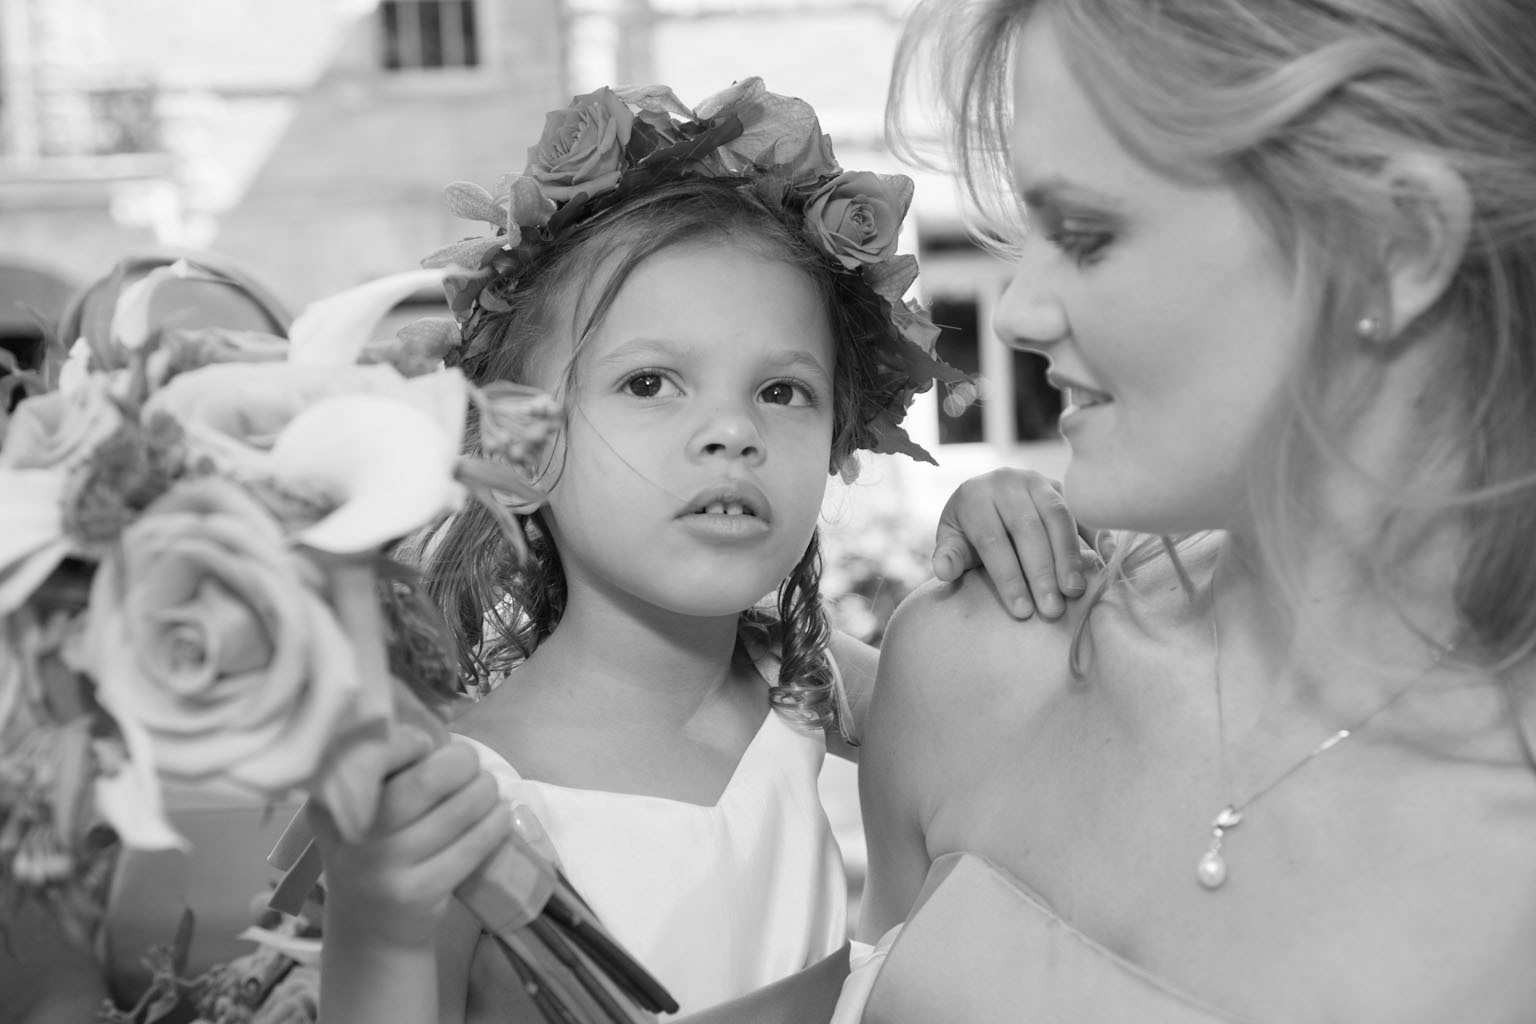
\includegraphics[width=0.8\textwidth]{blurb/hayley_and_heaven}
  \vspace{2\baselineskip}

  Heaven Malaika King-Bailey \\
  January 21\st, 2006 -- June 6\sth, 2010
  \vspace{2\baselineskip}

  What a bundle of joy. \\
  We'll miss you, love.
\end{center}
\end{dedications}

\begin{acknowledgments}
\epigraph{If I have seen further it is by standing on ye sholders of
  Giants.}{Isaac Newton\citep{turnbull59}}

Newton's competitive spirit gives the heroic phrasing in the quote
above, but I don't see the need to use giants (\cref{fig:ants}).  Any
furtherance of knowledge due to my research is due to consolidating,
reorganizing, and tweaking the work of those that came before me.  To
all of you in the rest of this innumerable bundle, thanks!

On a professional level, my high school physics teacher Tom Hoch
started this whole experience with a very engaging class, and I
continue to use his block counting analogy for energy conservation
when teaching new students.  Since then, I have been privileged to
work under Joe Amato, Dan Schult, Jeff Buboltz, the late Marc Feldman,
and the late Guoliang Yang, all of whom have helped mold me into the
scientist and person I am today.  Prof.~Yang deserves extra credit,
and his ability to shift topics from force spectroscopy to geopolitics
and back in a minute helped keep things fresh.  Thanks to Luis Cruz
Cruz for shepherding me through the final stages of my thesis.  My lab
partners Marisa Roman and Runcong Liu provided lively discussions and
a (mostly) willing audience for smoke testing my software.

On a personal level, my wife Emily and broader family and friends have
kept me sane throughout this process.  Thank you all.

Thanks to my committee members---Jian-Min Yuan, Jun Xi, Michel
Valli{\`e}res, Som Tyagi, and Prof.~Cruz---for helpful criticism and
review.  Also thanks to Mom, for lots of pro bono editing!  Any errors
that remain are clearly my fault, and corrections are
welcome\footnote{%
  Write me at \href{mailto:wking@tremily.us}{wking@tremily.us}.  You
  can browse the thesis source at
  \url{http://git.tremily.us/?p=thesis.git}.
}.

This work was produced using the following open source software projects:
\begin{description}
\item[\href{http://www.tug.org/texlive/}{\TeX live}/%
      \href{http://www.ctan.org/}{CTAN}]
  Typesetting.
\item[\href{http://sourceforge.net/projects/pgf/}{PGF}/%
      \href{http://asymptote.sourceforge.net/}{Asymptote}]
  Graphics programming.
\item[\href{http://www.python.org/}{Python}]
  General purpose scripting.
\item[\href{http://www.scons.org/}{SCons}]
  Build manager.
\item[\href{http://www.gnu.org/software/emacs/}{GNU Emacs}]
  Text editor.
\item[\href{http://git-scm.com/}{Git}]
  Version control.
\item[\href{http://www.gnu.org/}{GNU}/%
      \href{https://www.kernel.org/}{Linux}/%
      \href{http://www.gentoo.org/}{Gentoo}]
  Operating system and distribution.
\end{description}
and many, many more.  I am deeply indebted to all of the smart,
generous people who produce such wonderful tools.  Besides providing
the tools, they also provide very supportive communities to help haul
complete newbies like me up the learning curve.

\sawsim\ work was supported by National Institutes of Health Grants
R01-GM071793.

\begin{figure}
  \begin{center}
    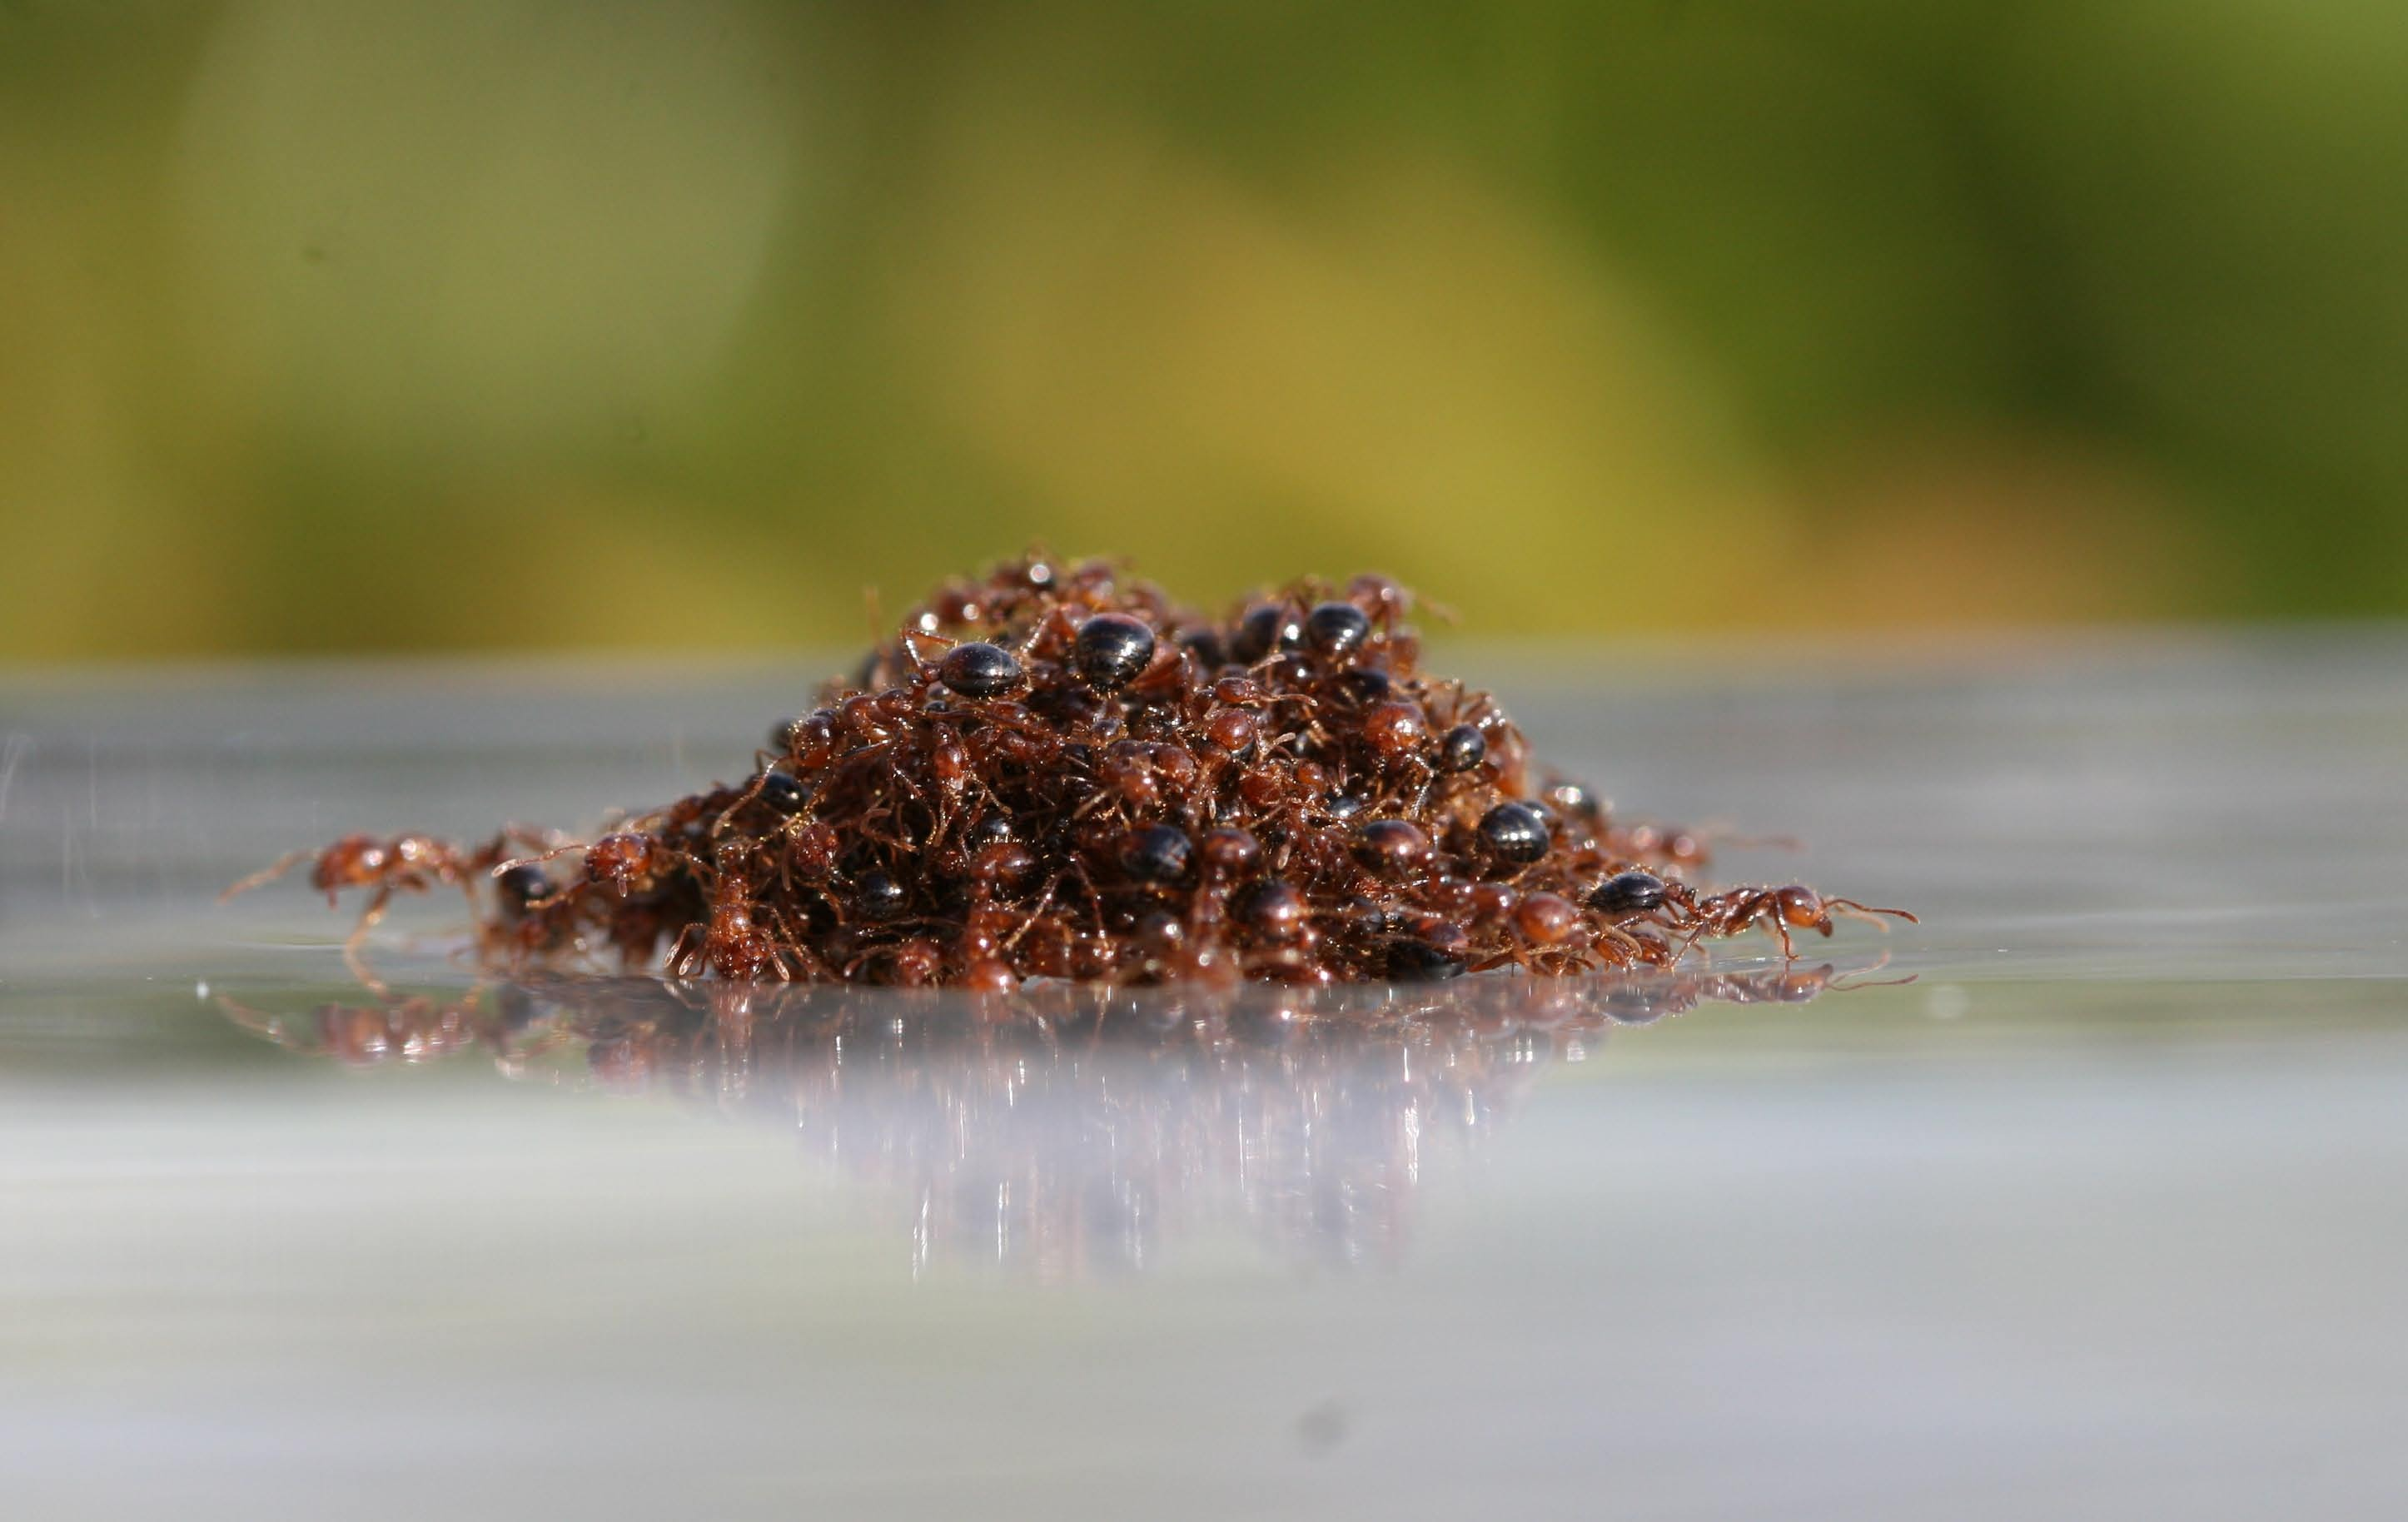
\includegraphics[width=4in]{figures/binary/ants}
    \caption{A raft of 500 fire ants, reproduced from
      \citet{mlot11}.\label{fig:ants}}
    \end{center}
\end{figure}
\end{acknowledgments}


\tableofcontents
\listoftables
\listoffigures

\begin{abstract}
Single molecule force spectroscopy (SMFS) experiments provide an
experimental benchmark for testing simulated and theoretical
predictions of protein unfolding behavior.  Despite it use since
1997\citep{rief97a}, the labs currently engaged in SMFS use in-house
software and procedures for critical tasks such as cantilever
calibration and Monte Carlo unfolding simulation.  Besides wasting
developer time producing and maintaining redundant implementations,
the lack of transparency makes it more difficult to share data and
techniques between labs, which slows progress.  In some cases it can
also lead to ambiguity as to which of several similar approaches,
correction factors, etc.\ were used in a particular paper.
%
\nomenclature[text ]{SMFS}{Single molecule force spectroscopy.}

In this thesis, I introduce an SMFS sofware suite for cantilever
calibration (\calibcant), experiment control (\unfoldprotein),
analysis (\Hooke), and postprocessing (\sawsim) in the context of
velocity clamp unfolding of I27 octomers in buffers with varying
concentrations of
\CaCl\citep{calibcant,unfold-protein,sandal09,king10}.  All of the
tools are licensed under open source licenses, which allows SMFS
researchers to centralize future development.  Where possible, care
has been taken to keep these packages operating system (OS) agnostic.
The experiment logic in \unfoldprotein\ and \calibcant\ is still
nominally OS agnostic, but those packages depend on more fundamental
packages that control the physical hardware in use\citep{pyafm}.  At
the bottom of the physical-interface stack are the \Comedi\ drivers
from the Linux kernel\citep{comedi}.  Users running other operating
systems should be able to swap in analogous low level
physical-interface packages if Linux is not an option.
%
\nomenclature[text ]{OS}{Operating system.}

\end{abstract}


\end{preamble}
\iffinal{}{\linenumbers}

\begin{thesis}
\pdfbookmark[-1]{Mainmatter}{Mainmatter}
\chapter{Introduction}
\label{sec:intro}

Single molecule force spectroscopy (SMFS) is the study of folding and
unfolding transitions in proteins under tension.  By measuring these
transitions, we hope to gain insight into fundamental protein
behavior.  SMFS is an attempt to bridge the gap between chemists
studying folding and unfolding kinetics in bulk solutions and
theorists simulating protein behavior at the amino-acid level.  An
increased understanding of protein folding would guide researchers in
developing drugs targeting biologically significant receptors and
enzymes.  In this chapter, I describe the protein folding problem in a
general sense (\cref{sec:folding-problem}), discuss theoretical
frameworks for understanding protein folding
(\cref{sec:energy-landscape}), highlight the role of SMFS in extending
this understanding (\cref{sec:single-molecule}), and explain the role
of unfolding experiments in understanding protein folding
(\cref{sec:unfolding}).  The last section in this chapter gives a
roadmap for the rest of the thesis (\cref{sec:outline}).

\section{The protein folding problem}
\label{sec:folding-problem}

% Why study protein folding?
In biological systems the most important molecules, such as proteins,
nucleic acids, and polysaccharides, are all polymers.  Understanding
the properties and functions of these polymeric molecules is crucial
in understanding the molecular mechanisms behind structures and
processes in cells.

% What do genes do?  Why is protein folding interesting?
An organism's genetic code is stored in DNA in the cell nucleus.
DNA sequencing is a fairly well developed field, with fundamental work
such as the Human Genome Project seeing major development in the early
2000s\citep{wolfsberg01,mcpherson01,collins03}.  It is estimated that
human genetic information contains approximately 25,000 genes, each
encoding a protein\citep{claverie01,venter01}.  Knowing the amino acid
sequence for a particular protein, however, does not immediately shed
light on the protein's role in the body, or even the protein's
probable conformation.  Indeed, a protein's conformation is often
vitally important in executing its biological tasks
(\cref{fig:ligand-receptor}).  Unfortunately predicting a protein's
stable conformations from it's amino acid sequence has proven to be
remarkably difficult, as has the inverse problem of finding sequences
that form a given conformation.
%
\nomenclature[text ]{DNA}{Deoxyribonucleic acid.}

\begin{figure}
  \begin{center}
  \includegraphics[width=2in]{figures/biotin-streptavidin/1SWE}%
  \caption{Complex of biotin\index{biotin} (red) and a
    streptavidin\index{streptavidin} tetramer (green)
    (\href{http://dx.doi.org/10.2210/pdb1swe/pdb}{PDB ID: 1SWE})%
    \citep{freitag97}.  The correct streptavidin conformation creates
    the biotin-specific binding pockets.  Biotin-streptavidin is a
    model ligand-receptor pair isolated from the bacterium
    \species{Streptomyces avidinii}%
    \index{Streptomyces@\species{Streptomyces avidnii}}.  Streptavidin
    binds to cell surfaces, and bound biotin increases streptavidin's
    cell-binding affinity\citep{alon90}.  Figure generated with
    \citetalias{pymol}.
    \label{fig:ligand-receptor}}
  \end{center}
\end{figure}


\section{Protein folding energy landscapes}
\label{sec:energy-landscape}

% the free energy landscape
Finding a protein's lowest energy state via a brute force sampling of
all possible conformations is impossibly inefficient, due to the
exponential scaling of possible conformations with protein length, as
outlined by \citet{levinthal69}.  This has lead to a succession of
models explaining the folding mechanism.  For a number of years, the
``pathway'' model of protein folding enjoyed popularity
(\cref{fig:folding:pathway})\citep{levinthal69}.  More recently, the
``landscape'' or ``funnel'' model has come to the fore
(\cref{fig:folding:landscape})\citep{dill97}.  Both of these models
reduce the conformation space to a more approachable analog, and their
success depends on striking a useful balance between simplicity and
accuracy.

\begin{figure}
  \begin{center}
  \subfloat[][]{
    \begin{tikzpicture}[->,node distance=1.5cm]
      \tikzstyle{every state}=[draw=white]
      \node[state] (U)                 {$U$};
      \node[state] (I1)  [right of=U]  {$I_1$};
      \node[state] (I1X) [below of=I1] {$I_1^X$};
      \node[state] (I2)  [right of=I1] {$I_2$};
      \node[state] (I2X) [below of=I2] {$I_2^X$};
      \node[state] (N)   [right of=I2] {$N$};
    
      \path[<->] (U)  edge (I1)
                 (I1) edge (I1X)
                 (I1) edge (I2)
                 (I2) edge (I2X)
                 (I2) edge (N);
    \end{tikzpicture}\label{fig:folding:pathway}}
  % \hspace{.25in}%
  \subfloat[][]{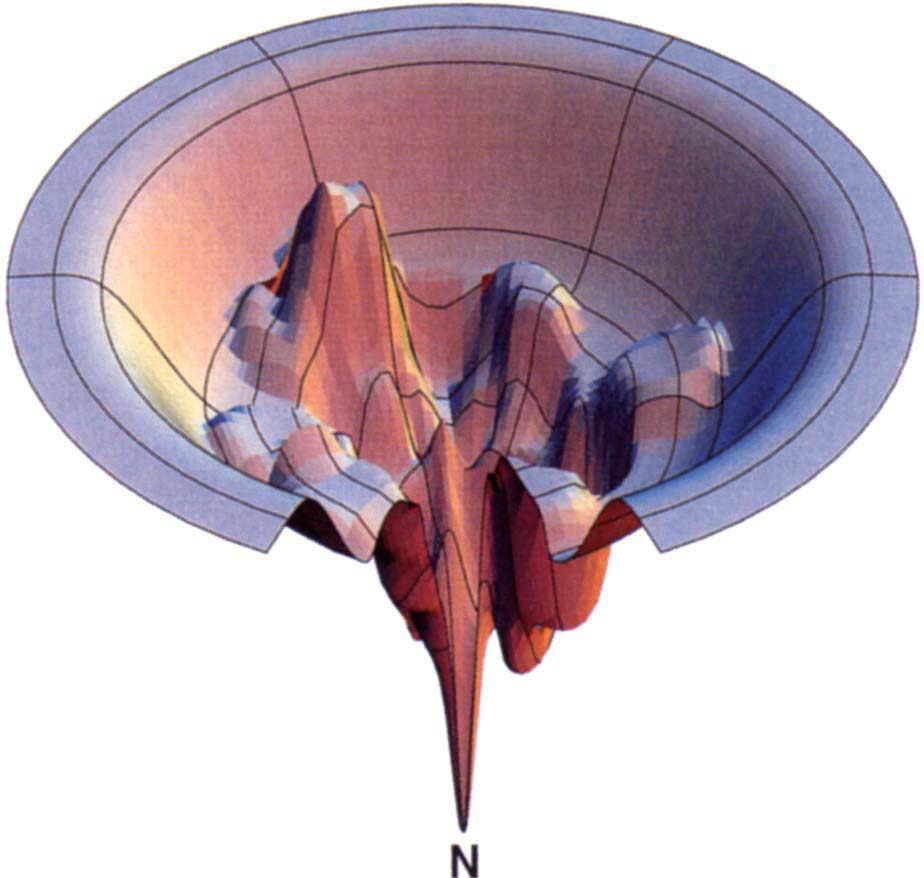
\includegraphics[width=2in]{figures/schematic/dill97-fig4}%
    \label{fig:folding:landscape}}
  \caption{\protect\subref{fig:folding:pathway} A ``double T'' example
    of the pathway model of protein folding, in which the protein
    proceeds from the native state $N$ to the unfolded state $U$ via a
    series of metastable transition states $I_1$ and $I_2$ with two
    ``dead end'' states $I_1^X$ and $I_2^X$.  Adapted from
    \citet{bedard08}.
    \protect\subref{fig:folding:landscape} The landscape model of
    protein folding, in which the protein diffuses through a
    multi-dimensional free energy landscape.  Separate folding
    attempts may take many distinct routes through this landscape on
    the way to the folded state.  Reproduced from
    \citet{dill97}.\label{fig:folding}}
  \end{center}
\end{figure}

When the choice of theoretical approach becomes murky, you must gather
experimental data to help distinguish between similar models.
Separating the pathway model from the funnel model is only marginally
within the realm of current experimental techniques, but with higher
throughput and increased automation it should be easier to make such
distinctions in the near future.


\section{Why \emph{single} molecule?}
\label{sec:single-molecule}

The large size of proteins relative to simpler molecules limits the
information attainable from bulk measurements, because the
macromolecules in a population can have diverse conformations and
behaviors.  Bulk measurements average over these differences,
producing excellent statistics for the mean, but making it difficult
to understand the variation.  The individualized, and sometimes rare,
behaviors of macromolecules can have important implications for their
functions inside the cell.  Single molecule techniques, in which the
macromolecules are studied one at a time, allow direct access to the
variation within the population without averaging.  This provides
important and complementary information about the functional
mechanisms of several biological systems\citep{bustamante08}.

Single molecule techniques provide an opportunity to study protein
folding and unfolding at the level of a single molecule, where the
distinction between the pathway model and funnel model is clearer.
They also provide a convenient benchmark for verifying molecular
dynamics simulations, because it takes lots of computing power to
simulate even one biopolymer with anything close to atomic resolution
over experimental time scales.  Even with significant computing
resources, comparing molecular dynamics results with experimental data
remains elusive.  For example, experimental pulling speeds are on the
order of \bareU{$\mu$m/s}, while simulation pulling speeds are on the
order of \bareU{m/s}\citep{lu98,lu99,rief02,zhao06,berkemeier11}.

% why AFM & what an AFM is
Single molecule techniques for manipulating biopolymers include
optical measurements, \ie, single molecule fluorescence microscopy and
spectroscopy, and mechanical manipulations of individual
macromolecules, \ie, force microscopy and spectroscopy using atomic
force microscopes (AFMs), laser tweezers\citep{kellermayer97,forde02},
magnetic tweezers\citep{smith92}, biomembrane force
probes\citep{merkel99}, and centrifugal
microscopes\citep{halvorsen09}.  These techniques cover a wide range
of approaches, and even when the basic approach is the same
(e.g.\ force microscopy), the different techniques span orders of
magnitude in the range of their controllable parameters.
%
\nomenclature[text ]{AFM}{Atomic force microscope (or microscopy).}

\section{Why \emph{un}folding?}
\label{sec:unfolding}

There's a lot of talk about protein \emph{folding} in this chapter,
while the rest of the thesis (and the title) are about
\emph{unfolding}.  If you understand protein folding, you can use your
understanding to design drugs with a particular conformation, or
predict the conformation of a biologically important receptor
(\cref{sec:folding-problem}).  Understanding protein unfolding is less
directly useful, because unfolded proteins are rarely biologically
relevant (although it does happen\citep{dyson05}).

The focus on unfolding is mainly because it's easier to unravel
proteins by pulling on their ends (\cref{sec:procedure}) than it is to
fold them into their native state by pushing on those ends
(\cref{fig:ligand-receptor,fig:I27}).  For proteins with smooth enough
energy landscapes, the folding and unfolding routes will be similar,
so knowledge about the unfolding behavior \emph{does} shed light on
the folding behavior.

Practically, the distinction between folding and unfolding makes
little difference, because drug designers and doctors are not
consuming SMFS results directly.  For researchers calibrating
molecular dynamics simulations, it doesn't matter if you compare
simulated folding experiments with experimental folding experiments,
or simulated unfolding experiments with experimental unfolding
experiments.  The important thing is to compare your simulation
against \emph{some} experimental benchmarks.  If your molecular
dynamics simulation successfully predicts a protein's unfolding
behavior, it makes me more confident that it will correctly predict
the protein's native folding behavior.


\section{Thesis outline}
\label{sec:outline}

\Cref{sec:methods} of this thesis outlines the apparatus and methods
for single molecule force spectroscopy with an atomic force
microscope.  \Cref{sec:sawsim} presents my \sawsim\ Monte Carlo
simulation for modeling unfolding/refolding behavior.  By comparing
model simulations with experimental measurements, we can gain insight
into the protein's kinetics.  After \cref{sec:sawsim}, you should have
a pretty firm grasp of the underlying physics, so we'll move on to
\cref{sec:pyafm} and discuss my \pyafm\ and \unfoldprotein\ experiment
control software.  With both the kinetic theory and procedure taken
care of, \cref{sec:calibcant} discusses thermal cantilever
calibration, deriving the theoretical approach and presenting my
\calibcant\ automatic calibration software.

Moving away from experiment control, \cref{sec:hooke} presents the
\Hooke\ suite for extracting unfolding force histograms (for
comparison with \sawsim\ simulations).  In \cref{sec:salt}, I pull all
the pieces together (experiment control, post processing, and
simulation) to carry out unfolding experiments on the
immunoglobulin-like domain 27 from human Titin (I27) in buffers with
different ionic strength.  We close with \cref{sec:future}, which
summarizes my conclusions and discusses possible directions for future
work.

\chapter{Introduction}
\label{sec:intro}

Single molecule force spectroscopy (SMFS) is the study of folding and
unfolding transitions in proteins under tension.  By measuring these
transitions, we hope to gain insight into fundamental protein
behavior.  SMFS is an attempt to bridge the gap between chemists
studying folding and unfolding kinetics in bulk solutions and
theorists simulating protein behavior at the amino-acid level.  An
increased understanding of protein folding would guide researchers in
developing drugs targeting biologically significant receptors and
enzymes.  In this chapter, I describe the protein folding problem in a
general sense (\cref{sec:folding-problem}), discuss theoretical
frameworks for understanding protein folding
(\cref{sec:energy-landscape}), highlight the role of SMFS in extending
this understanding (\cref{sec:single-molecule}), and explain the role
of unfolding experiments in understanding protein folding
(\cref{sec:unfolding}).  The last section in this chapter gives a
roadmap for the rest of the thesis (\cref{sec:outline}).

\section{The protein folding problem}
\label{sec:folding-problem}

% Why study protein folding?
In biological systems the most important molecules, such as proteins,
nucleic acids, and polysaccharides, are all polymers.  Understanding
the properties and functions of these polymeric molecules is crucial
in understanding the molecular mechanisms behind structures and
processes in cells.

% What do genes do?  Why is protein folding interesting?
An organism's genetic code is stored in DNA in the cell nucleus.
DNA sequencing is a fairly well developed field, with fundamental work
such as the Human Genome Project seeing major development in the early
2000s\citep{wolfsberg01,mcpherson01,collins03}.  It is estimated that
human genetic information contains approximately 25,000 genes, each
encoding a protein\citep{claverie01,venter01}.  Knowing the amino acid
sequence for a particular protein, however, does not immediately shed
light on the protein's role in the body, or even the protein's
probable conformation.  Indeed, a protein's conformation is often
vitally important in executing its biological tasks
(\cref{fig:ligand-receptor}).  Unfortunately predicting a protein's
stable conformations from it's amino acid sequence has proven to be
remarkably difficult, as has the inverse problem of finding sequences
that form a given conformation.
%
\nomenclature[text ]{DNA}{Deoxyribonucleic acid.}

\begin{figure}
  \begin{center}
  \includegraphics[width=2in]{figures/biotin-streptavidin/1SWE}%
  \caption{Complex of biotin\index{biotin} (red) and a
    streptavidin\index{streptavidin} tetramer (green)
    (\href{http://dx.doi.org/10.2210/pdb1swe/pdb}{PDB ID: 1SWE})%
    \citep{freitag97}.  The correct streptavidin conformation creates
    the biotin-specific binding pockets.  Biotin-streptavidin is a
    model ligand-receptor pair isolated from the bacterium
    \species{Streptomyces avidinii}%
    \index{Streptomyces@\species{Streptomyces avidnii}}.  Streptavidin
    binds to cell surfaces, and bound biotin increases streptavidin's
    cell-binding affinity\citep{alon90}.  Figure generated with
    \citetalias{pymol}.
    \label{fig:ligand-receptor}}
  \end{center}
\end{figure}


\section{Protein folding energy landscapes}
\label{sec:energy-landscape}

% the free energy landscape
Finding a protein's lowest energy state via a brute force sampling of
all possible conformations is impossibly inefficient, due to the
exponential scaling of possible conformations with protein length, as
outlined by \citet{levinthal69}.  This has lead to a succession of
models explaining the folding mechanism.  For a number of years, the
``pathway'' model of protein folding enjoyed popularity
(\cref{fig:folding:pathway})\citep{levinthal69}.  More recently, the
``landscape'' or ``funnel'' model has come to the fore
(\cref{fig:folding:landscape})\citep{dill97}.  Both of these models
reduce the conformation space to a more approachable analog, and their
success depends on striking a useful balance between simplicity and
accuracy.

\begin{figure}
  \begin{center}
  \subfloat[][]{
    \begin{tikzpicture}[->,node distance=1.5cm]
      \tikzstyle{every state}=[draw=white]
      \node[state] (U)                 {$U$};
      \node[state] (I1)  [right of=U]  {$I_1$};
      \node[state] (I1X) [below of=I1] {$I_1^X$};
      \node[state] (I2)  [right of=I1] {$I_2$};
      \node[state] (I2X) [below of=I2] {$I_2^X$};
      \node[state] (N)   [right of=I2] {$N$};
    
      \path[<->] (U)  edge (I1)
                 (I1) edge (I1X)
                 (I1) edge (I2)
                 (I2) edge (I2X)
                 (I2) edge (N);
    \end{tikzpicture}\label{fig:folding:pathway}}
  % \hspace{.25in}%
  \subfloat[][]{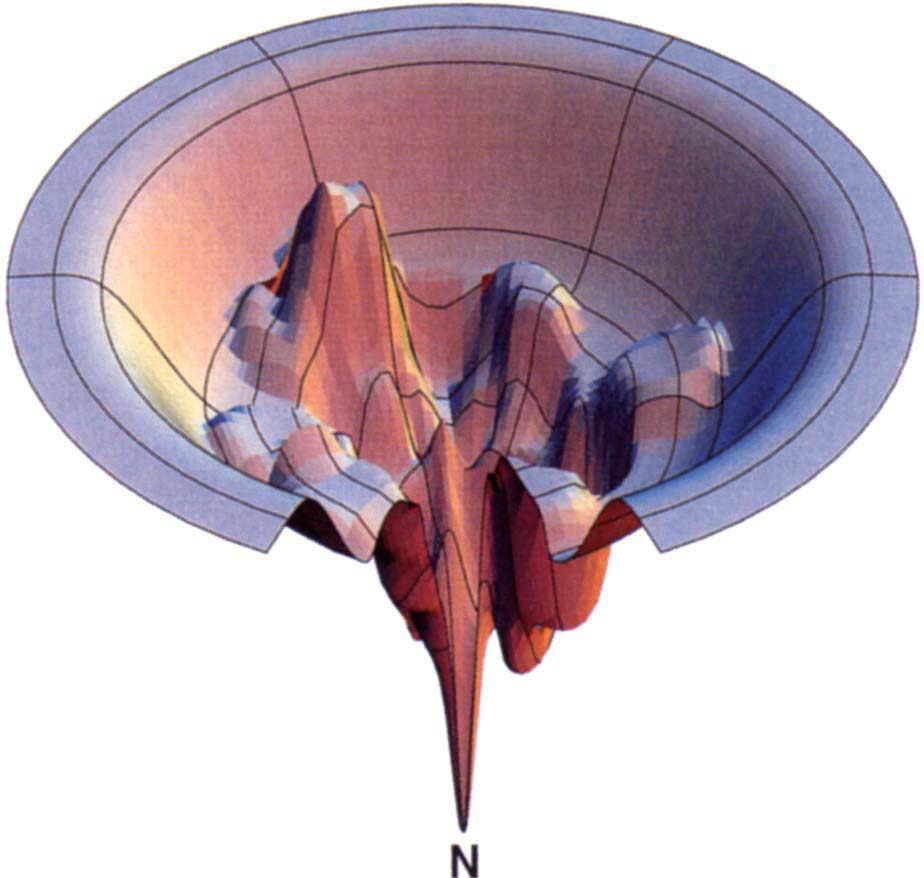
\includegraphics[width=2in]{figures/schematic/dill97-fig4}%
    \label{fig:folding:landscape}}
  \caption{\protect\subref{fig:folding:pathway} A ``double T'' example
    of the pathway model of protein folding, in which the protein
    proceeds from the native state $N$ to the unfolded state $U$ via a
    series of metastable transition states $I_1$ and $I_2$ with two
    ``dead end'' states $I_1^X$ and $I_2^X$.  Adapted from
    \citet{bedard08}.
    \protect\subref{fig:folding:landscape} The landscape model of
    protein folding, in which the protein diffuses through a
    multi-dimensional free energy landscape.  Separate folding
    attempts may take many distinct routes through this landscape on
    the way to the folded state.  Reproduced from
    \citet{dill97}.\label{fig:folding}}
  \end{center}
\end{figure}

When the choice of theoretical approach becomes murky, you must gather
experimental data to help distinguish between similar models.
Separating the pathway model from the funnel model is only marginally
within the realm of current experimental techniques, but with higher
throughput and increased automation it should be easier to make such
distinctions in the near future.


\section{Why \emph{single} molecule?}
\label{sec:single-molecule}

The large size of proteins relative to simpler molecules limits the
information attainable from bulk measurements, because the
macromolecules in a population can have diverse conformations and
behaviors.  Bulk measurements average over these differences,
producing excellent statistics for the mean, but making it difficult
to understand the variation.  The individualized, and sometimes rare,
behaviors of macromolecules can have important implications for their
functions inside the cell.  Single molecule techniques, in which the
macromolecules are studied one at a time, allow direct access to the
variation within the population without averaging.  This provides
important and complementary information about the functional
mechanisms of several biological systems\citep{bustamante08}.

Single molecule techniques provide an opportunity to study protein
folding and unfolding at the level of a single molecule, where the
distinction between the pathway model and funnel model is clearer.
They also provide a convenient benchmark for verifying molecular
dynamics simulations, because it takes lots of computing power to
simulate even one biopolymer with anything close to atomic resolution
over experimental time scales.  Even with significant computing
resources, comparing molecular dynamics results with experimental data
remains elusive.  For example, experimental pulling speeds are on the
order of \bareU{$\mu$m/s}, while simulation pulling speeds are on the
order of \bareU{m/s}\citep{lu98,lu99,rief02,zhao06,berkemeier11}.

% why AFM & what an AFM is
Single molecule techniques for manipulating biopolymers include
optical measurements, \ie, single molecule fluorescence microscopy and
spectroscopy, and mechanical manipulations of individual
macromolecules, \ie, force microscopy and spectroscopy using atomic
force microscopes (AFMs), laser tweezers\citep{kellermayer97,forde02},
magnetic tweezers\citep{smith92}, biomembrane force
probes\citep{merkel99}, and centrifugal
microscopes\citep{halvorsen09}.  These techniques cover a wide range
of approaches, and even when the basic approach is the same
(e.g.\ force microscopy), the different techniques span orders of
magnitude in the range of their controllable parameters.
%
\nomenclature[text ]{AFM}{Atomic force microscope (or microscopy).}

\section{Why \emph{un}folding?}
\label{sec:unfolding}

There's a lot of talk about protein \emph{folding} in this chapter,
while the rest of the thesis (and the title) are about
\emph{unfolding}.  If you understand protein folding, you can use your
understanding to design drugs with a particular conformation, or
predict the conformation of a biologically important receptor
(\cref{sec:folding-problem}).  Understanding protein unfolding is less
directly useful, because unfolded proteins are rarely biologically
relevant (although it does happen\citep{dyson05}).

The focus on unfolding is mainly because it's easier to unravel
proteins by pulling on their ends (\cref{sec:procedure}) than it is to
fold them into their native state by pushing on those ends
(\cref{fig:ligand-receptor,fig:I27}).  For proteins with smooth enough
energy landscapes, the folding and unfolding routes will be similar,
so knowledge about the unfolding behavior \emph{does} shed light on
the folding behavior.

Practically, the distinction between folding and unfolding makes
little difference, because drug designers and doctors are not
consuming SMFS results directly.  For researchers calibrating
molecular dynamics simulations, it doesn't matter if you compare
simulated folding experiments with experimental folding experiments,
or simulated unfolding experiments with experimental unfolding
experiments.  The important thing is to compare your simulation
against \emph{some} experimental benchmarks.  If your molecular
dynamics simulation successfully predicts a protein's unfolding
behavior, it makes me more confident that it will correctly predict
the protein's native folding behavior.


\section{Thesis outline}
\label{sec:outline}

\Cref{sec:methods} of this thesis outlines the apparatus and methods
for single molecule force spectroscopy with an atomic force
microscope.  \Cref{sec:sawsim} presents my \sawsim\ Monte Carlo
simulation for modeling unfolding/refolding behavior.  By comparing
model simulations with experimental measurements, we can gain insight
into the protein's kinetics.  After \cref{sec:sawsim}, you should have
a pretty firm grasp of the underlying physics, so we'll move on to
\cref{sec:pyafm} and discuss my \pyafm\ and \unfoldprotein\ experiment
control software.  With both the kinetic theory and procedure taken
care of, \cref{sec:calibcant} discusses thermal cantilever
calibration, deriving the theoretical approach and presenting my
\calibcant\ automatic calibration software.

Moving away from experiment control, \cref{sec:hooke} presents the
\Hooke\ suite for extracting unfolding force histograms (for
comparison with \sawsim\ simulations).  In \cref{sec:salt}, I pull all
the pieces together (experiment control, post processing, and
simulation) to carry out unfolding experiments on the
immunoglobulin-like domain 27 from human Titin (I27) in buffers with
different ionic strength.  We close with \cref{sec:future}, which
summarizes my conclusions and discusses possible directions for future
work.

\chapter{Introduction}
\label{sec:intro}

Single molecule force spectroscopy (SMFS) is the study of folding and
unfolding transitions in proteins under tension.  By measuring these
transitions, we hope to gain insight into fundamental protein
behavior.  SMFS is an attempt to bridge the gap between chemists
studying folding and unfolding kinetics in bulk solutions and
theorists simulating protein behavior at the amino-acid level.  An
increased understanding of protein folding would guide researchers in
developing drugs targeting biologically significant receptors and
enzymes.  In this chapter, I describe the protein folding problem in a
general sense (\cref{sec:folding-problem}), discuss theoretical
frameworks for understanding protein folding
(\cref{sec:energy-landscape}), highlight the role of SMFS in extending
this understanding (\cref{sec:single-molecule}), and explain the role
of unfolding experiments in understanding protein folding
(\cref{sec:unfolding}).  The last section in this chapter gives a
roadmap for the rest of the thesis (\cref{sec:outline}).

\section{The protein folding problem}
\label{sec:folding-problem}

% Why study protein folding?
In biological systems the most important molecules, such as proteins,
nucleic acids, and polysaccharides, are all polymers.  Understanding
the properties and functions of these polymeric molecules is crucial
in understanding the molecular mechanisms behind structures and
processes in cells.

% What do genes do?  Why is protein folding interesting?
An organism's genetic code is stored in DNA in the cell nucleus.
DNA sequencing is a fairly well developed field, with fundamental work
such as the Human Genome Project seeing major development in the early
2000s\citep{wolfsberg01,mcpherson01,collins03}.  It is estimated that
human genetic information contains approximately 25,000 genes, each
encoding a protein\citep{claverie01,venter01}.  Knowing the amino acid
sequence for a particular protein, however, does not immediately shed
light on the protein's role in the body, or even the protein's
probable conformation.  Indeed, a protein's conformation is often
vitally important in executing its biological tasks
(\cref{fig:ligand-receptor}).  Unfortunately predicting a protein's
stable conformations from it's amino acid sequence has proven to be
remarkably difficult, as has the inverse problem of finding sequences
that form a given conformation.
%
\nomenclature[text ]{DNA}{Deoxyribonucleic acid.}

\begin{figure}
  \begin{center}
  \includegraphics[width=2in]{figures/biotin-streptavidin/1SWE}%
  \caption{Complex of biotin\index{biotin} (red) and a
    streptavidin\index{streptavidin} tetramer (green)
    (\href{http://dx.doi.org/10.2210/pdb1swe/pdb}{PDB ID: 1SWE})%
    \citep{freitag97}.  The correct streptavidin conformation creates
    the biotin-specific binding pockets.  Biotin-streptavidin is a
    model ligand-receptor pair isolated from the bacterium
    \species{Streptomyces avidinii}%
    \index{Streptomyces@\species{Streptomyces avidnii}}.  Streptavidin
    binds to cell surfaces, and bound biotin increases streptavidin's
    cell-binding affinity\citep{alon90}.  Figure generated with
    \citetalias{pymol}.
    \label{fig:ligand-receptor}}
  \end{center}
\end{figure}


\section{Protein folding energy landscapes}
\label{sec:energy-landscape}

% the free energy landscape
Finding a protein's lowest energy state via a brute force sampling of
all possible conformations is impossibly inefficient, due to the
exponential scaling of possible conformations with protein length, as
outlined by \citet{levinthal69}.  This has lead to a succession of
models explaining the folding mechanism.  For a number of years, the
``pathway'' model of protein folding enjoyed popularity
(\cref{fig:folding:pathway})\citep{levinthal69}.  More recently, the
``landscape'' or ``funnel'' model has come to the fore
(\cref{fig:folding:landscape})\citep{dill97}.  Both of these models
reduce the conformation space to a more approachable analog, and their
success depends on striking a useful balance between simplicity and
accuracy.

\begin{figure}
  \begin{center}
  \subfloat[][]{
    \begin{tikzpicture}[->,node distance=1.5cm]
      \tikzstyle{every state}=[draw=white]
      \node[state] (U)                 {$U$};
      \node[state] (I1)  [right of=U]  {$I_1$};
      \node[state] (I1X) [below of=I1] {$I_1^X$};
      \node[state] (I2)  [right of=I1] {$I_2$};
      \node[state] (I2X) [below of=I2] {$I_2^X$};
      \node[state] (N)   [right of=I2] {$N$};
    
      \path[<->] (U)  edge (I1)
                 (I1) edge (I1X)
                 (I1) edge (I2)
                 (I2) edge (I2X)
                 (I2) edge (N);
    \end{tikzpicture}\label{fig:folding:pathway}}
  % \hspace{.25in}%
  \subfloat[][]{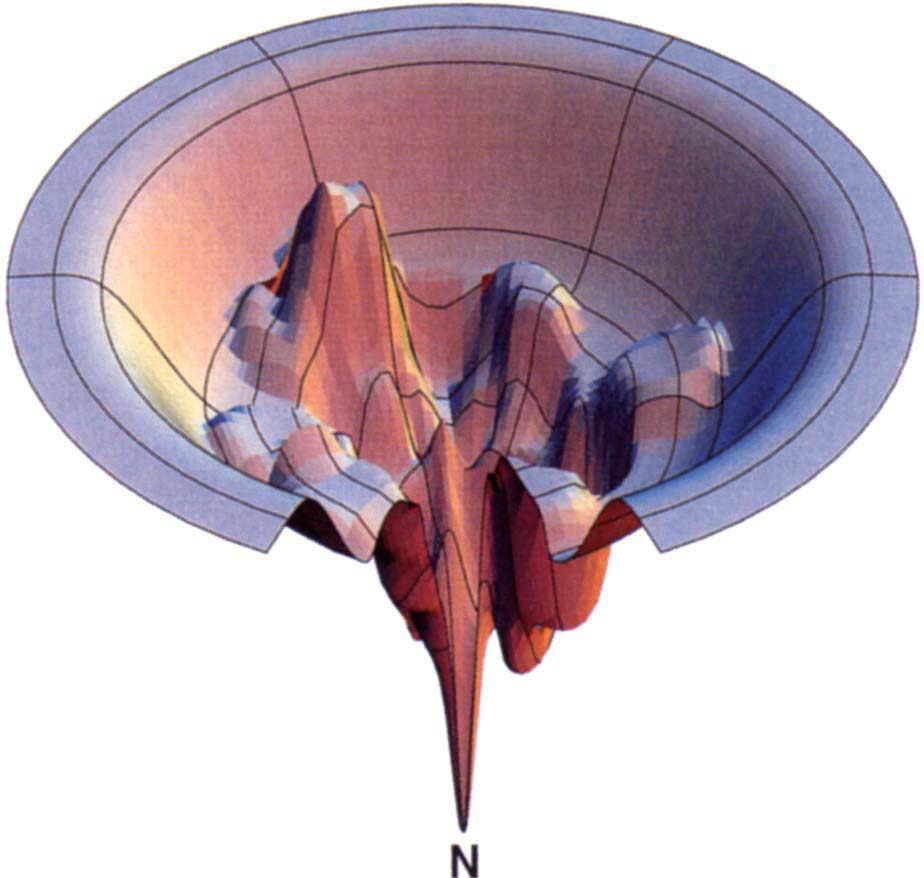
\includegraphics[width=2in]{figures/schematic/dill97-fig4}%
    \label{fig:folding:landscape}}
  \caption{\protect\subref{fig:folding:pathway} A ``double T'' example
    of the pathway model of protein folding, in which the protein
    proceeds from the native state $N$ to the unfolded state $U$ via a
    series of metastable transition states $I_1$ and $I_2$ with two
    ``dead end'' states $I_1^X$ and $I_2^X$.  Adapted from
    \citet{bedard08}.
    \protect\subref{fig:folding:landscape} The landscape model of
    protein folding, in which the protein diffuses through a
    multi-dimensional free energy landscape.  Separate folding
    attempts may take many distinct routes through this landscape on
    the way to the folded state.  Reproduced from
    \citet{dill97}.\label{fig:folding}}
  \end{center}
\end{figure}

When the choice of theoretical approach becomes murky, you must gather
experimental data to help distinguish between similar models.
Separating the pathway model from the funnel model is only marginally
within the realm of current experimental techniques, but with higher
throughput and increased automation it should be easier to make such
distinctions in the near future.


\section{Why \emph{single} molecule?}
\label{sec:single-molecule}

The large size of proteins relative to simpler molecules limits the
information attainable from bulk measurements, because the
macromolecules in a population can have diverse conformations and
behaviors.  Bulk measurements average over these differences,
producing excellent statistics for the mean, but making it difficult
to understand the variation.  The individualized, and sometimes rare,
behaviors of macromolecules can have important implications for their
functions inside the cell.  Single molecule techniques, in which the
macromolecules are studied one at a time, allow direct access to the
variation within the population without averaging.  This provides
important and complementary information about the functional
mechanisms of several biological systems\citep{bustamante08}.

Single molecule techniques provide an opportunity to study protein
folding and unfolding at the level of a single molecule, where the
distinction between the pathway model and funnel model is clearer.
They also provide a convenient benchmark for verifying molecular
dynamics simulations, because it takes lots of computing power to
simulate even one biopolymer with anything close to atomic resolution
over experimental time scales.  Even with significant computing
resources, comparing molecular dynamics results with experimental data
remains elusive.  For example, experimental pulling speeds are on the
order of \bareU{$\mu$m/s}, while simulation pulling speeds are on the
order of \bareU{m/s}\citep{lu98,lu99,rief02,zhao06,berkemeier11}.

% why AFM & what an AFM is
Single molecule techniques for manipulating biopolymers include
optical measurements, \ie, single molecule fluorescence microscopy and
spectroscopy, and mechanical manipulations of individual
macromolecules, \ie, force microscopy and spectroscopy using atomic
force microscopes (AFMs), laser tweezers\citep{kellermayer97,forde02},
magnetic tweezers\citep{smith92}, biomembrane force
probes\citep{merkel99}, and centrifugal
microscopes\citep{halvorsen09}.  These techniques cover a wide range
of approaches, and even when the basic approach is the same
(e.g.\ force microscopy), the different techniques span orders of
magnitude in the range of their controllable parameters.
%
\nomenclature[text ]{AFM}{Atomic force microscope (or microscopy).}

\section{Why \emph{un}folding?}
\label{sec:unfolding}

There's a lot of talk about protein \emph{folding} in this chapter,
while the rest of the thesis (and the title) are about
\emph{unfolding}.  If you understand protein folding, you can use your
understanding to design drugs with a particular conformation, or
predict the conformation of a biologically important receptor
(\cref{sec:folding-problem}).  Understanding protein unfolding is less
directly useful, because unfolded proteins are rarely biologically
relevant (although it does happen\citep{dyson05}).

The focus on unfolding is mainly because it's easier to unravel
proteins by pulling on their ends (\cref{sec:procedure}) than it is to
fold them into their native state by pushing on those ends
(\cref{fig:ligand-receptor,fig:I27}).  For proteins with smooth enough
energy landscapes, the folding and unfolding routes will be similar,
so knowledge about the unfolding behavior \emph{does} shed light on
the folding behavior.

Practically, the distinction between folding and unfolding makes
little difference, because drug designers and doctors are not
consuming SMFS results directly.  For researchers calibrating
molecular dynamics simulations, it doesn't matter if you compare
simulated folding experiments with experimental folding experiments,
or simulated unfolding experiments with experimental unfolding
experiments.  The important thing is to compare your simulation
against \emph{some} experimental benchmarks.  If your molecular
dynamics simulation successfully predicts a protein's unfolding
behavior, it makes me more confident that it will correctly predict
the protein's native folding behavior.


\section{Thesis outline}
\label{sec:outline}

\Cref{sec:methods} of this thesis outlines the apparatus and methods
for single molecule force spectroscopy with an atomic force
microscope.  \Cref{sec:sawsim} presents my \sawsim\ Monte Carlo
simulation for modeling unfolding/refolding behavior.  By comparing
model simulations with experimental measurements, we can gain insight
into the protein's kinetics.  After \cref{sec:sawsim}, you should have
a pretty firm grasp of the underlying physics, so we'll move on to
\cref{sec:pyafm} and discuss my \pyafm\ and \unfoldprotein\ experiment
control software.  With both the kinetic theory and procedure taken
care of, \cref{sec:calibcant} discusses thermal cantilever
calibration, deriving the theoretical approach and presenting my
\calibcant\ automatic calibration software.

Moving away from experiment control, \cref{sec:hooke} presents the
\Hooke\ suite for extracting unfolding force histograms (for
comparison with \sawsim\ simulations).  In \cref{sec:salt}, I pull all
the pieces together (experiment control, post processing, and
simulation) to carry out unfolding experiments on the
immunoglobulin-like domain 27 from human Titin (I27) in buffers with
different ionic strength.  We close with \cref{sec:future}, which
summarizes my conclusions and discusses possible directions for future
work.

\chapter{Introduction}
\label{sec:intro}

Single molecule force spectroscopy (SMFS) is the study of folding and
unfolding transitions in proteins under tension.  By measuring these
transitions, we hope to gain insight into fundamental protein
behavior.  SMFS is an attempt to bridge the gap between chemists
studying folding and unfolding kinetics in bulk solutions and
theorists simulating protein behavior at the amino-acid level.  An
increased understanding of protein folding would guide researchers in
developing drugs targeting biologically significant receptors and
enzymes.  In this chapter, I describe the protein folding problem in a
general sense (\cref{sec:folding-problem}), discuss theoretical
frameworks for understanding protein folding
(\cref{sec:energy-landscape}), highlight the role of SMFS in extending
this understanding (\cref{sec:single-molecule}), and explain the role
of unfolding experiments in understanding protein folding
(\cref{sec:unfolding}).  The last section in this chapter gives a
roadmap for the rest of the thesis (\cref{sec:outline}).

\section{The protein folding problem}
\label{sec:folding-problem}

% Why study protein folding?
In biological systems the most important molecules, such as proteins,
nucleic acids, and polysaccharides, are all polymers.  Understanding
the properties and functions of these polymeric molecules is crucial
in understanding the molecular mechanisms behind structures and
processes in cells.

% What do genes do?  Why is protein folding interesting?
An organism's genetic code is stored in DNA in the cell nucleus.
DNA sequencing is a fairly well developed field, with fundamental work
such as the Human Genome Project seeing major development in the early
2000s\citep{wolfsberg01,mcpherson01,collins03}.  It is estimated that
human genetic information contains approximately 25,000 genes, each
encoding a protein\citep{claverie01,venter01}.  Knowing the amino acid
sequence for a particular protein, however, does not immediately shed
light on the protein's role in the body, or even the protein's
probable conformation.  Indeed, a protein's conformation is often
vitally important in executing its biological tasks
(\cref{fig:ligand-receptor}).  Unfortunately predicting a protein's
stable conformations from it's amino acid sequence has proven to be
remarkably difficult, as has the inverse problem of finding sequences
that form a given conformation.
%
\nomenclature[text ]{DNA}{Deoxyribonucleic acid.}

\begin{figure}
  \begin{center}
  \includegraphics[width=2in]{figures/biotin-streptavidin/1SWE}%
  \caption{Complex of biotin\index{biotin} (red) and a
    streptavidin\index{streptavidin} tetramer (green)
    (\href{http://dx.doi.org/10.2210/pdb1swe/pdb}{PDB ID: 1SWE})%
    \citep{freitag97}.  The correct streptavidin conformation creates
    the biotin-specific binding pockets.  Biotin-streptavidin is a
    model ligand-receptor pair isolated from the bacterium
    \species{Streptomyces avidinii}%
    \index{Streptomyces@\species{Streptomyces avidnii}}.  Streptavidin
    binds to cell surfaces, and bound biotin increases streptavidin's
    cell-binding affinity\citep{alon90}.  Figure generated with
    \citetalias{pymol}.
    \label{fig:ligand-receptor}}
  \end{center}
\end{figure}


\section{Protein folding energy landscapes}
\label{sec:energy-landscape}

% the free energy landscape
Finding a protein's lowest energy state via a brute force sampling of
all possible conformations is impossibly inefficient, due to the
exponential scaling of possible conformations with protein length, as
outlined by \citet{levinthal69}.  This has lead to a succession of
models explaining the folding mechanism.  For a number of years, the
``pathway'' model of protein folding enjoyed popularity
(\cref{fig:folding:pathway})\citep{levinthal69}.  More recently, the
``landscape'' or ``funnel'' model has come to the fore
(\cref{fig:folding:landscape})\citep{dill97}.  Both of these models
reduce the conformation space to a more approachable analog, and their
success depends on striking a useful balance between simplicity and
accuracy.

\begin{figure}
  \begin{center}
  \subfloat[][]{
    \begin{tikzpicture}[->,node distance=1.5cm]
      \tikzstyle{every state}=[draw=white]
      \node[state] (U)                 {$U$};
      \node[state] (I1)  [right of=U]  {$I_1$};
      \node[state] (I1X) [below of=I1] {$I_1^X$};
      \node[state] (I2)  [right of=I1] {$I_2$};
      \node[state] (I2X) [below of=I2] {$I_2^X$};
      \node[state] (N)   [right of=I2] {$N$};
    
      \path[<->] (U)  edge (I1)
                 (I1) edge (I1X)
                 (I1) edge (I2)
                 (I2) edge (I2X)
                 (I2) edge (N);
    \end{tikzpicture}\label{fig:folding:pathway}}
  % \hspace{.25in}%
  \subfloat[][]{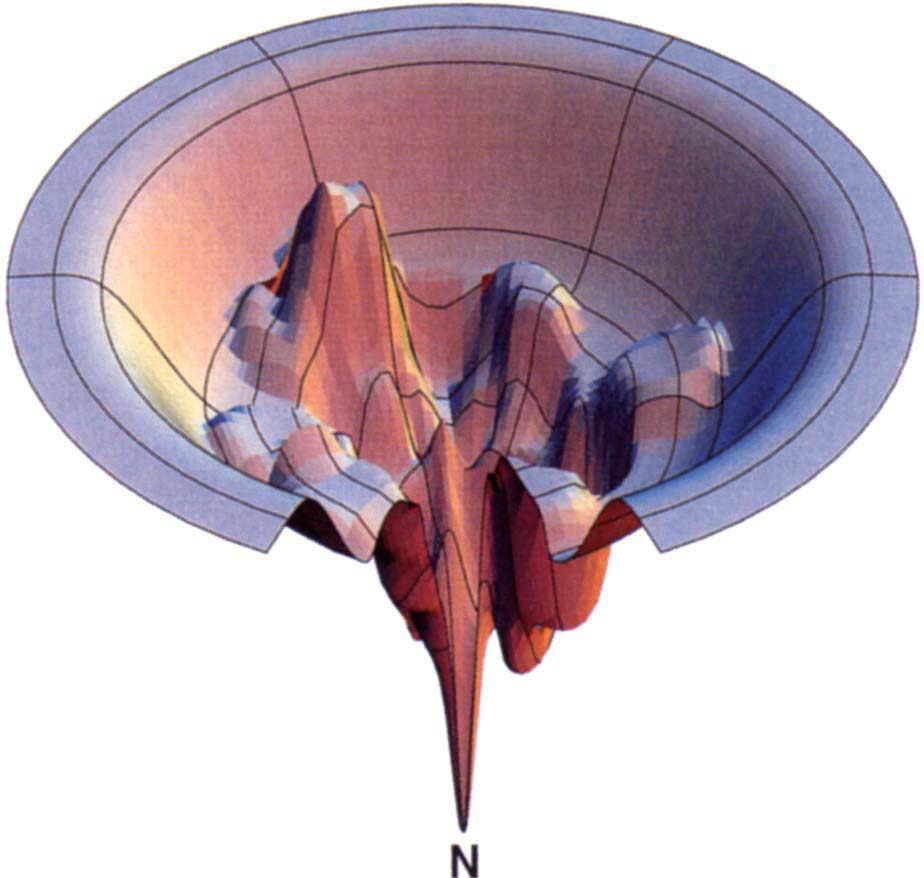
\includegraphics[width=2in]{figures/schematic/dill97-fig4}%
    \label{fig:folding:landscape}}
  \caption{\protect\subref{fig:folding:pathway} A ``double T'' example
    of the pathway model of protein folding, in which the protein
    proceeds from the native state $N$ to the unfolded state $U$ via a
    series of metastable transition states $I_1$ and $I_2$ with two
    ``dead end'' states $I_1^X$ and $I_2^X$.  Adapted from
    \citet{bedard08}.
    \protect\subref{fig:folding:landscape} The landscape model of
    protein folding, in which the protein diffuses through a
    multi-dimensional free energy landscape.  Separate folding
    attempts may take many distinct routes through this landscape on
    the way to the folded state.  Reproduced from
    \citet{dill97}.\label{fig:folding}}
  \end{center}
\end{figure}

When the choice of theoretical approach becomes murky, you must gather
experimental data to help distinguish between similar models.
Separating the pathway model from the funnel model is only marginally
within the realm of current experimental techniques, but with higher
throughput and increased automation it should be easier to make such
distinctions in the near future.


\section{Why \emph{single} molecule?}
\label{sec:single-molecule}

The large size of proteins relative to simpler molecules limits the
information attainable from bulk measurements, because the
macromolecules in a population can have diverse conformations and
behaviors.  Bulk measurements average over these differences,
producing excellent statistics for the mean, but making it difficult
to understand the variation.  The individualized, and sometimes rare,
behaviors of macromolecules can have important implications for their
functions inside the cell.  Single molecule techniques, in which the
macromolecules are studied one at a time, allow direct access to the
variation within the population without averaging.  This provides
important and complementary information about the functional
mechanisms of several biological systems\citep{bustamante08}.

Single molecule techniques provide an opportunity to study protein
folding and unfolding at the level of a single molecule, where the
distinction between the pathway model and funnel model is clearer.
They also provide a convenient benchmark for verifying molecular
dynamics simulations, because it takes lots of computing power to
simulate even one biopolymer with anything close to atomic resolution
over experimental time scales.  Even with significant computing
resources, comparing molecular dynamics results with experimental data
remains elusive.  For example, experimental pulling speeds are on the
order of \bareU{$\mu$m/s}, while simulation pulling speeds are on the
order of \bareU{m/s}\citep{lu98,lu99,rief02,zhao06,berkemeier11}.

% why AFM & what an AFM is
Single molecule techniques for manipulating biopolymers include
optical measurements, \ie, single molecule fluorescence microscopy and
spectroscopy, and mechanical manipulations of individual
macromolecules, \ie, force microscopy and spectroscopy using atomic
force microscopes (AFMs), laser tweezers\citep{kellermayer97,forde02},
magnetic tweezers\citep{smith92}, biomembrane force
probes\citep{merkel99}, and centrifugal
microscopes\citep{halvorsen09}.  These techniques cover a wide range
of approaches, and even when the basic approach is the same
(e.g.\ force microscopy), the different techniques span orders of
magnitude in the range of their controllable parameters.
%
\nomenclature[text ]{AFM}{Atomic force microscope (or microscopy).}

\section{Why \emph{un}folding?}
\label{sec:unfolding}

There's a lot of talk about protein \emph{folding} in this chapter,
while the rest of the thesis (and the title) are about
\emph{unfolding}.  If you understand protein folding, you can use your
understanding to design drugs with a particular conformation, or
predict the conformation of a biologically important receptor
(\cref{sec:folding-problem}).  Understanding protein unfolding is less
directly useful, because unfolded proteins are rarely biologically
relevant (although it does happen\citep{dyson05}).

The focus on unfolding is mainly because it's easier to unravel
proteins by pulling on their ends (\cref{sec:procedure}) than it is to
fold them into their native state by pushing on those ends
(\cref{fig:ligand-receptor,fig:I27}).  For proteins with smooth enough
energy landscapes, the folding and unfolding routes will be similar,
so knowledge about the unfolding behavior \emph{does} shed light on
the folding behavior.

Practically, the distinction between folding and unfolding makes
little difference, because drug designers and doctors are not
consuming SMFS results directly.  For researchers calibrating
molecular dynamics simulations, it doesn't matter if you compare
simulated folding experiments with experimental folding experiments,
or simulated unfolding experiments with experimental unfolding
experiments.  The important thing is to compare your simulation
against \emph{some} experimental benchmarks.  If your molecular
dynamics simulation successfully predicts a protein's unfolding
behavior, it makes me more confident that it will correctly predict
the protein's native folding behavior.


\section{Thesis outline}
\label{sec:outline}

\Cref{sec:methods} of this thesis outlines the apparatus and methods
for single molecule force spectroscopy with an atomic force
microscope.  \Cref{sec:sawsim} presents my \sawsim\ Monte Carlo
simulation for modeling unfolding/refolding behavior.  By comparing
model simulations with experimental measurements, we can gain insight
into the protein's kinetics.  After \cref{sec:sawsim}, you should have
a pretty firm grasp of the underlying physics, so we'll move on to
\cref{sec:pyafm} and discuss my \pyafm\ and \unfoldprotein\ experiment
control software.  With both the kinetic theory and procedure taken
care of, \cref{sec:calibcant} discusses thermal cantilever
calibration, deriving the theoretical approach and presenting my
\calibcant\ automatic calibration software.

Moving away from experiment control, \cref{sec:hooke} presents the
\Hooke\ suite for extracting unfolding force histograms (for
comparison with \sawsim\ simulations).  In \cref{sec:salt}, I pull all
the pieces together (experiment control, post processing, and
simulation) to carry out unfolding experiments on the
immunoglobulin-like domain 27 from human Titin (I27) in buffers with
different ionic strength.  We close with \cref{sec:future}, which
summarizes my conclusions and discusses possible directions for future
work.

\chapter{Introduction}
\label{sec:intro}

Single molecule force spectroscopy (SMFS) is the study of folding and
unfolding transitions in proteins under tension.  By measuring these
transitions, we hope to gain insight into fundamental protein
behavior.  SMFS is an attempt to bridge the gap between chemists
studying folding and unfolding kinetics in bulk solutions and
theorists simulating protein behavior at the amino-acid level.  An
increased understanding of protein folding would guide researchers in
developing drugs targeting biologically significant receptors and
enzymes.  In this chapter, I describe the protein folding problem in a
general sense (\cref{sec:folding-problem}), discuss theoretical
frameworks for understanding protein folding
(\cref{sec:energy-landscape}), highlight the role of SMFS in extending
this understanding (\cref{sec:single-molecule}), and explain the role
of unfolding experiments in understanding protein folding
(\cref{sec:unfolding}).  The last section in this chapter gives a
roadmap for the rest of the thesis (\cref{sec:outline}).

\section{The protein folding problem}
\label{sec:folding-problem}

% Why study protein folding?
In biological systems the most important molecules, such as proteins,
nucleic acids, and polysaccharides, are all polymers.  Understanding
the properties and functions of these polymeric molecules is crucial
in understanding the molecular mechanisms behind structures and
processes in cells.

% What do genes do?  Why is protein folding interesting?
An organism's genetic code is stored in DNA in the cell nucleus.
DNA sequencing is a fairly well developed field, with fundamental work
such as the Human Genome Project seeing major development in the early
2000s\citep{wolfsberg01,mcpherson01,collins03}.  It is estimated that
human genetic information contains approximately 25,000 genes, each
encoding a protein\citep{claverie01,venter01}.  Knowing the amino acid
sequence for a particular protein, however, does not immediately shed
light on the protein's role in the body, or even the protein's
probable conformation.  Indeed, a protein's conformation is often
vitally important in executing its biological tasks
(\cref{fig:ligand-receptor}).  Unfortunately predicting a protein's
stable conformations from it's amino acid sequence has proven to be
remarkably difficult, as has the inverse problem of finding sequences
that form a given conformation.
%
\nomenclature[text ]{DNA}{Deoxyribonucleic acid.}

\begin{figure}
  \begin{center}
  \includegraphics[width=2in]{figures/biotin-streptavidin/1SWE}%
  \caption{Complex of biotin\index{biotin} (red) and a
    streptavidin\index{streptavidin} tetramer (green)
    (\href{http://dx.doi.org/10.2210/pdb1swe/pdb}{PDB ID: 1SWE})%
    \citep{freitag97}.  The correct streptavidin conformation creates
    the biotin-specific binding pockets.  Biotin-streptavidin is a
    model ligand-receptor pair isolated from the bacterium
    \species{Streptomyces avidinii}%
    \index{Streptomyces@\species{Streptomyces avidnii}}.  Streptavidin
    binds to cell surfaces, and bound biotin increases streptavidin's
    cell-binding affinity\citep{alon90}.  Figure generated with
    \citetalias{pymol}.
    \label{fig:ligand-receptor}}
  \end{center}
\end{figure}


\section{Protein folding energy landscapes}
\label{sec:energy-landscape}

% the free energy landscape
Finding a protein's lowest energy state via a brute force sampling of
all possible conformations is impossibly inefficient, due to the
exponential scaling of possible conformations with protein length, as
outlined by \citet{levinthal69}.  This has lead to a succession of
models explaining the folding mechanism.  For a number of years, the
``pathway'' model of protein folding enjoyed popularity
(\cref{fig:folding:pathway})\citep{levinthal69}.  More recently, the
``landscape'' or ``funnel'' model has come to the fore
(\cref{fig:folding:landscape})\citep{dill97}.  Both of these models
reduce the conformation space to a more approachable analog, and their
success depends on striking a useful balance between simplicity and
accuracy.

\begin{figure}
  \begin{center}
  \subfloat[][]{
    \begin{tikzpicture}[->,node distance=1.5cm]
      \tikzstyle{every state}=[draw=white]
      \node[state] (U)                 {$U$};
      \node[state] (I1)  [right of=U]  {$I_1$};
      \node[state] (I1X) [below of=I1] {$I_1^X$};
      \node[state] (I2)  [right of=I1] {$I_2$};
      \node[state] (I2X) [below of=I2] {$I_2^X$};
      \node[state] (N)   [right of=I2] {$N$};
    
      \path[<->] (U)  edge (I1)
                 (I1) edge (I1X)
                 (I1) edge (I2)
                 (I2) edge (I2X)
                 (I2) edge (N);
    \end{tikzpicture}\label{fig:folding:pathway}}
  % \hspace{.25in}%
  \subfloat[][]{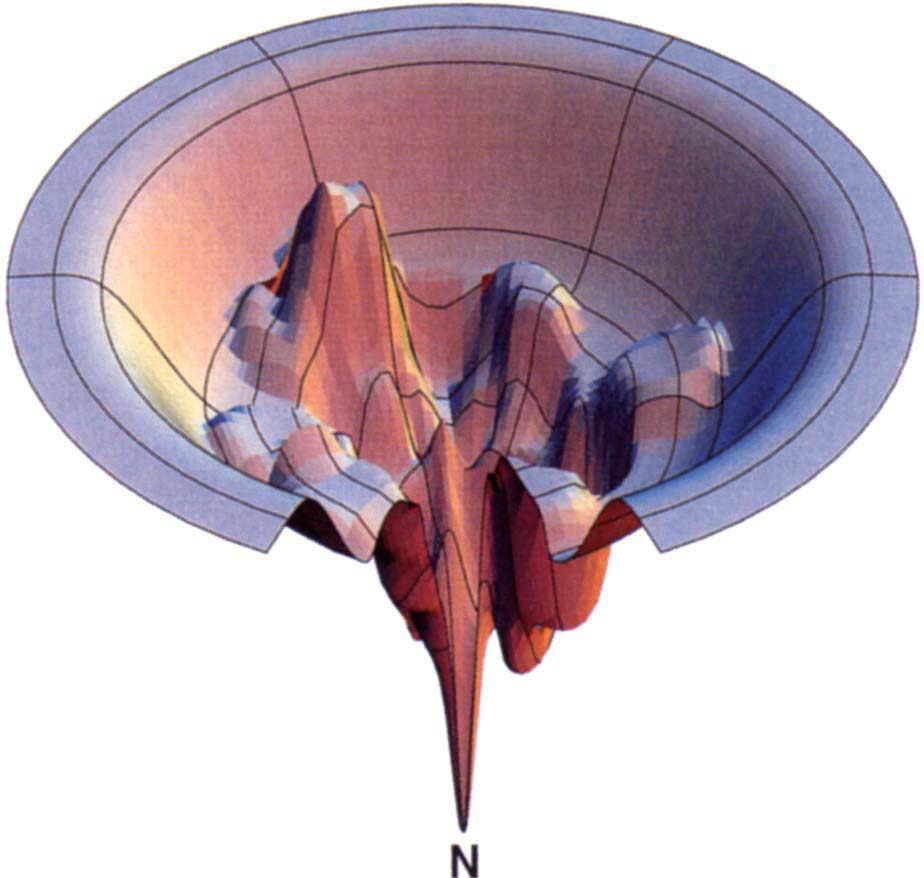
\includegraphics[width=2in]{figures/schematic/dill97-fig4}%
    \label{fig:folding:landscape}}
  \caption{\protect\subref{fig:folding:pathway} A ``double T'' example
    of the pathway model of protein folding, in which the protein
    proceeds from the native state $N$ to the unfolded state $U$ via a
    series of metastable transition states $I_1$ and $I_2$ with two
    ``dead end'' states $I_1^X$ and $I_2^X$.  Adapted from
    \citet{bedard08}.
    \protect\subref{fig:folding:landscape} The landscape model of
    protein folding, in which the protein diffuses through a
    multi-dimensional free energy landscape.  Separate folding
    attempts may take many distinct routes through this landscape on
    the way to the folded state.  Reproduced from
    \citet{dill97}.\label{fig:folding}}
  \end{center}
\end{figure}

When the choice of theoretical approach becomes murky, you must gather
experimental data to help distinguish between similar models.
Separating the pathway model from the funnel model is only marginally
within the realm of current experimental techniques, but with higher
throughput and increased automation it should be easier to make such
distinctions in the near future.


\section{Why \emph{single} molecule?}
\label{sec:single-molecule}

The large size of proteins relative to simpler molecules limits the
information attainable from bulk measurements, because the
macromolecules in a population can have diverse conformations and
behaviors.  Bulk measurements average over these differences,
producing excellent statistics for the mean, but making it difficult
to understand the variation.  The individualized, and sometimes rare,
behaviors of macromolecules can have important implications for their
functions inside the cell.  Single molecule techniques, in which the
macromolecules are studied one at a time, allow direct access to the
variation within the population without averaging.  This provides
important and complementary information about the functional
mechanisms of several biological systems\citep{bustamante08}.

Single molecule techniques provide an opportunity to study protein
folding and unfolding at the level of a single molecule, where the
distinction between the pathway model and funnel model is clearer.
They also provide a convenient benchmark for verifying molecular
dynamics simulations, because it takes lots of computing power to
simulate even one biopolymer with anything close to atomic resolution
over experimental time scales.  Even with significant computing
resources, comparing molecular dynamics results with experimental data
remains elusive.  For example, experimental pulling speeds are on the
order of \bareU{$\mu$m/s}, while simulation pulling speeds are on the
order of \bareU{m/s}\citep{lu98,lu99,rief02,zhao06,berkemeier11}.

% why AFM & what an AFM is
Single molecule techniques for manipulating biopolymers include
optical measurements, \ie, single molecule fluorescence microscopy and
spectroscopy, and mechanical manipulations of individual
macromolecules, \ie, force microscopy and spectroscopy using atomic
force microscopes (AFMs), laser tweezers\citep{kellermayer97,forde02},
magnetic tweezers\citep{smith92}, biomembrane force
probes\citep{merkel99}, and centrifugal
microscopes\citep{halvorsen09}.  These techniques cover a wide range
of approaches, and even when the basic approach is the same
(e.g.\ force microscopy), the different techniques span orders of
magnitude in the range of their controllable parameters.
%
\nomenclature[text ]{AFM}{Atomic force microscope (or microscopy).}

\section{Why \emph{un}folding?}
\label{sec:unfolding}

There's a lot of talk about protein \emph{folding} in this chapter,
while the rest of the thesis (and the title) are about
\emph{unfolding}.  If you understand protein folding, you can use your
understanding to design drugs with a particular conformation, or
predict the conformation of a biologically important receptor
(\cref{sec:folding-problem}).  Understanding protein unfolding is less
directly useful, because unfolded proteins are rarely biologically
relevant (although it does happen\citep{dyson05}).

The focus on unfolding is mainly because it's easier to unravel
proteins by pulling on their ends (\cref{sec:procedure}) than it is to
fold them into their native state by pushing on those ends
(\cref{fig:ligand-receptor,fig:I27}).  For proteins with smooth enough
energy landscapes, the folding and unfolding routes will be similar,
so knowledge about the unfolding behavior \emph{does} shed light on
the folding behavior.

Practically, the distinction between folding and unfolding makes
little difference, because drug designers and doctors are not
consuming SMFS results directly.  For researchers calibrating
molecular dynamics simulations, it doesn't matter if you compare
simulated folding experiments with experimental folding experiments,
or simulated unfolding experiments with experimental unfolding
experiments.  The important thing is to compare your simulation
against \emph{some} experimental benchmarks.  If your molecular
dynamics simulation successfully predicts a protein's unfolding
behavior, it makes me more confident that it will correctly predict
the protein's native folding behavior.


\section{Thesis outline}
\label{sec:outline}

\Cref{sec:methods} of this thesis outlines the apparatus and methods
for single molecule force spectroscopy with an atomic force
microscope.  \Cref{sec:sawsim} presents my \sawsim\ Monte Carlo
simulation for modeling unfolding/refolding behavior.  By comparing
model simulations with experimental measurements, we can gain insight
into the protein's kinetics.  After \cref{sec:sawsim}, you should have
a pretty firm grasp of the underlying physics, so we'll move on to
\cref{sec:pyafm} and discuss my \pyafm\ and \unfoldprotein\ experiment
control software.  With both the kinetic theory and procedure taken
care of, \cref{sec:calibcant} discusses thermal cantilever
calibration, deriving the theoretical approach and presenting my
\calibcant\ automatic calibration software.

Moving away from experiment control, \cref{sec:hooke} presents the
\Hooke\ suite for extracting unfolding force histograms (for
comparison with \sawsim\ simulations).  In \cref{sec:salt}, I pull all
the pieces together (experiment control, post processing, and
simulation) to carry out unfolding experiments on the
immunoglobulin-like domain 27 from human Titin (I27) in buffers with
different ionic strength.  We close with \cref{sec:future}, which
summarizes my conclusions and discusses possible directions for future
work.

\chapter{Introduction}
\label{sec:intro}

Single molecule force spectroscopy (SMFS) is the study of folding and
unfolding transitions in proteins under tension.  By measuring these
transitions, we hope to gain insight into fundamental protein
behavior.  SMFS is an attempt to bridge the gap between chemists
studying folding and unfolding kinetics in bulk solutions and
theorists simulating protein behavior at the amino-acid level.  An
increased understanding of protein folding would guide researchers in
developing drugs targeting biologically significant receptors and
enzymes.  In this chapter, I describe the protein folding problem in a
general sense (\cref{sec:folding-problem}), discuss theoretical
frameworks for understanding protein folding
(\cref{sec:energy-landscape}), highlight the role of SMFS in extending
this understanding (\cref{sec:single-molecule}), and explain the role
of unfolding experiments in understanding protein folding
(\cref{sec:unfolding}).  The last section in this chapter gives a
roadmap for the rest of the thesis (\cref{sec:outline}).

\section{The protein folding problem}
\label{sec:folding-problem}

% Why study protein folding?
In biological systems the most important molecules, such as proteins,
nucleic acids, and polysaccharides, are all polymers.  Understanding
the properties and functions of these polymeric molecules is crucial
in understanding the molecular mechanisms behind structures and
processes in cells.

% What do genes do?  Why is protein folding interesting?
An organism's genetic code is stored in DNA in the cell nucleus.
DNA sequencing is a fairly well developed field, with fundamental work
such as the Human Genome Project seeing major development in the early
2000s\citep{wolfsberg01,mcpherson01,collins03}.  It is estimated that
human genetic information contains approximately 25,000 genes, each
encoding a protein\citep{claverie01,venter01}.  Knowing the amino acid
sequence for a particular protein, however, does not immediately shed
light on the protein's role in the body, or even the protein's
probable conformation.  Indeed, a protein's conformation is often
vitally important in executing its biological tasks
(\cref{fig:ligand-receptor}).  Unfortunately predicting a protein's
stable conformations from it's amino acid sequence has proven to be
remarkably difficult, as has the inverse problem of finding sequences
that form a given conformation.
%
\nomenclature[text ]{DNA}{Deoxyribonucleic acid.}

\begin{figure}
  \begin{center}
  \includegraphics[width=2in]{figures/biotin-streptavidin/1SWE}%
  \caption{Complex of biotin\index{biotin} (red) and a
    streptavidin\index{streptavidin} tetramer (green)
    (\href{http://dx.doi.org/10.2210/pdb1swe/pdb}{PDB ID: 1SWE})%
    \citep{freitag97}.  The correct streptavidin conformation creates
    the biotin-specific binding pockets.  Biotin-streptavidin is a
    model ligand-receptor pair isolated from the bacterium
    \species{Streptomyces avidinii}%
    \index{Streptomyces@\species{Streptomyces avidnii}}.  Streptavidin
    binds to cell surfaces, and bound biotin increases streptavidin's
    cell-binding affinity\citep{alon90}.  Figure generated with
    \citetalias{pymol}.
    \label{fig:ligand-receptor}}
  \end{center}
\end{figure}


\section{Protein folding energy landscapes}
\label{sec:energy-landscape}

% the free energy landscape
Finding a protein's lowest energy state via a brute force sampling of
all possible conformations is impossibly inefficient, due to the
exponential scaling of possible conformations with protein length, as
outlined by \citet{levinthal69}.  This has lead to a succession of
models explaining the folding mechanism.  For a number of years, the
``pathway'' model of protein folding enjoyed popularity
(\cref{fig:folding:pathway})\citep{levinthal69}.  More recently, the
``landscape'' or ``funnel'' model has come to the fore
(\cref{fig:folding:landscape})\citep{dill97}.  Both of these models
reduce the conformation space to a more approachable analog, and their
success depends on striking a useful balance between simplicity and
accuracy.

\begin{figure}
  \begin{center}
  \subfloat[][]{
    \begin{tikzpicture}[->,node distance=1.5cm]
      \tikzstyle{every state}=[draw=white]
      \node[state] (U)                 {$U$};
      \node[state] (I1)  [right of=U]  {$I_1$};
      \node[state] (I1X) [below of=I1] {$I_1^X$};
      \node[state] (I2)  [right of=I1] {$I_2$};
      \node[state] (I2X) [below of=I2] {$I_2^X$};
      \node[state] (N)   [right of=I2] {$N$};
    
      \path[<->] (U)  edge (I1)
                 (I1) edge (I1X)
                 (I1) edge (I2)
                 (I2) edge (I2X)
                 (I2) edge (N);
    \end{tikzpicture}\label{fig:folding:pathway}}
  % \hspace{.25in}%
  \subfloat[][]{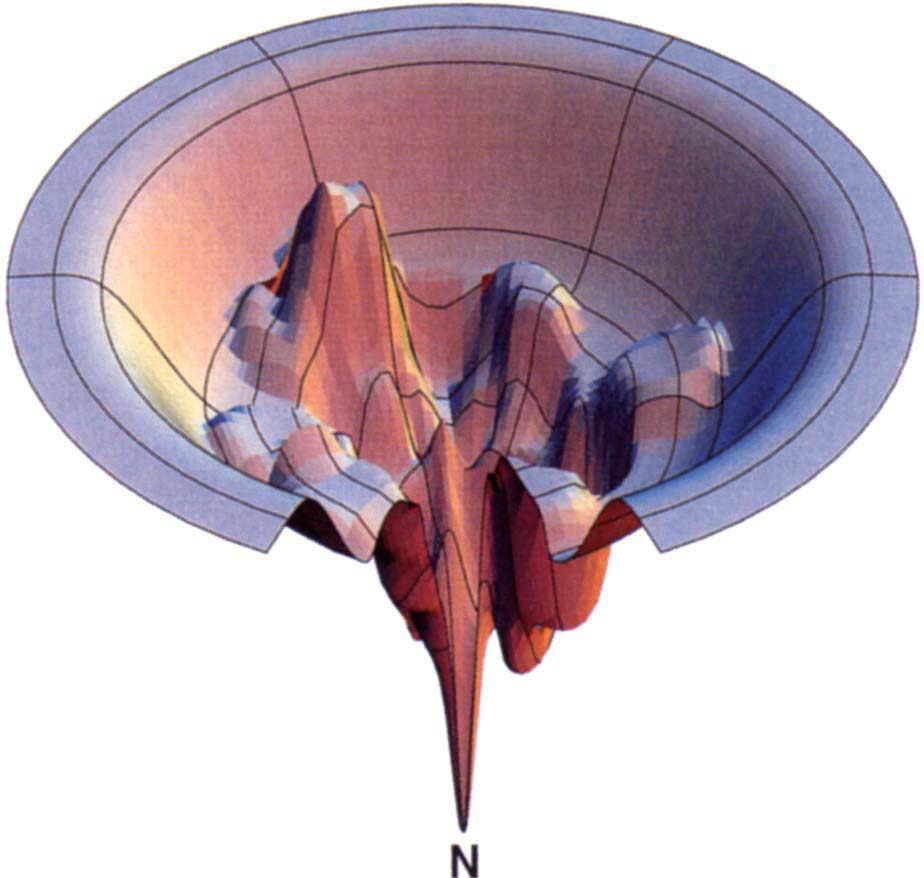
\includegraphics[width=2in]{figures/schematic/dill97-fig4}%
    \label{fig:folding:landscape}}
  \caption{\protect\subref{fig:folding:pathway} A ``double T'' example
    of the pathway model of protein folding, in which the protein
    proceeds from the native state $N$ to the unfolded state $U$ via a
    series of metastable transition states $I_1$ and $I_2$ with two
    ``dead end'' states $I_1^X$ and $I_2^X$.  Adapted from
    \citet{bedard08}.
    \protect\subref{fig:folding:landscape} The landscape model of
    protein folding, in which the protein diffuses through a
    multi-dimensional free energy landscape.  Separate folding
    attempts may take many distinct routes through this landscape on
    the way to the folded state.  Reproduced from
    \citet{dill97}.\label{fig:folding}}
  \end{center}
\end{figure}

When the choice of theoretical approach becomes murky, you must gather
experimental data to help distinguish between similar models.
Separating the pathway model from the funnel model is only marginally
within the realm of current experimental techniques, but with higher
throughput and increased automation it should be easier to make such
distinctions in the near future.


\section{Why \emph{single} molecule?}
\label{sec:single-molecule}

The large size of proteins relative to simpler molecules limits the
information attainable from bulk measurements, because the
macromolecules in a population can have diverse conformations and
behaviors.  Bulk measurements average over these differences,
producing excellent statistics for the mean, but making it difficult
to understand the variation.  The individualized, and sometimes rare,
behaviors of macromolecules can have important implications for their
functions inside the cell.  Single molecule techniques, in which the
macromolecules are studied one at a time, allow direct access to the
variation within the population without averaging.  This provides
important and complementary information about the functional
mechanisms of several biological systems\citep{bustamante08}.

Single molecule techniques provide an opportunity to study protein
folding and unfolding at the level of a single molecule, where the
distinction between the pathway model and funnel model is clearer.
They also provide a convenient benchmark for verifying molecular
dynamics simulations, because it takes lots of computing power to
simulate even one biopolymer with anything close to atomic resolution
over experimental time scales.  Even with significant computing
resources, comparing molecular dynamics results with experimental data
remains elusive.  For example, experimental pulling speeds are on the
order of \bareU{$\mu$m/s}, while simulation pulling speeds are on the
order of \bareU{m/s}\citep{lu98,lu99,rief02,zhao06,berkemeier11}.

% why AFM & what an AFM is
Single molecule techniques for manipulating biopolymers include
optical measurements, \ie, single molecule fluorescence microscopy and
spectroscopy, and mechanical manipulations of individual
macromolecules, \ie, force microscopy and spectroscopy using atomic
force microscopes (AFMs), laser tweezers\citep{kellermayer97,forde02},
magnetic tweezers\citep{smith92}, biomembrane force
probes\citep{merkel99}, and centrifugal
microscopes\citep{halvorsen09}.  These techniques cover a wide range
of approaches, and even when the basic approach is the same
(e.g.\ force microscopy), the different techniques span orders of
magnitude in the range of their controllable parameters.
%
\nomenclature[text ]{AFM}{Atomic force microscope (or microscopy).}

\section{Why \emph{un}folding?}
\label{sec:unfolding}

There's a lot of talk about protein \emph{folding} in this chapter,
while the rest of the thesis (and the title) are about
\emph{unfolding}.  If you understand protein folding, you can use your
understanding to design drugs with a particular conformation, or
predict the conformation of a biologically important receptor
(\cref{sec:folding-problem}).  Understanding protein unfolding is less
directly useful, because unfolded proteins are rarely biologically
relevant (although it does happen\citep{dyson05}).

The focus on unfolding is mainly because it's easier to unravel
proteins by pulling on their ends (\cref{sec:procedure}) than it is to
fold them into their native state by pushing on those ends
(\cref{fig:ligand-receptor,fig:I27}).  For proteins with smooth enough
energy landscapes, the folding and unfolding routes will be similar,
so knowledge about the unfolding behavior \emph{does} shed light on
the folding behavior.

Practically, the distinction between folding and unfolding makes
little difference, because drug designers and doctors are not
consuming SMFS results directly.  For researchers calibrating
molecular dynamics simulations, it doesn't matter if you compare
simulated folding experiments with experimental folding experiments,
or simulated unfolding experiments with experimental unfolding
experiments.  The important thing is to compare your simulation
against \emph{some} experimental benchmarks.  If your molecular
dynamics simulation successfully predicts a protein's unfolding
behavior, it makes me more confident that it will correctly predict
the protein's native folding behavior.


\section{Thesis outline}
\label{sec:outline}

\Cref{sec:methods} of this thesis outlines the apparatus and methods
for single molecule force spectroscopy with an atomic force
microscope.  \Cref{sec:sawsim} presents my \sawsim\ Monte Carlo
simulation for modeling unfolding/refolding behavior.  By comparing
model simulations with experimental measurements, we can gain insight
into the protein's kinetics.  After \cref{sec:sawsim}, you should have
a pretty firm grasp of the underlying physics, so we'll move on to
\cref{sec:pyafm} and discuss my \pyafm\ and \unfoldprotein\ experiment
control software.  With both the kinetic theory and procedure taken
care of, \cref{sec:calibcant} discusses thermal cantilever
calibration, deriving the theoretical approach and presenting my
\calibcant\ automatic calibration software.

Moving away from experiment control, \cref{sec:hooke} presents the
\Hooke\ suite for extracting unfolding force histograms (for
comparison with \sawsim\ simulations).  In \cref{sec:salt}, I pull all
the pieces together (experiment control, post processing, and
simulation) to carry out unfolding experiments on the
immunoglobulin-like domain 27 from human Titin (I27) in buffers with
different ionic strength.  We close with \cref{sec:future}, which
summarizes my conclusions and discusses possible directions for future
work.

%\chapter{Introduction}
\label{sec:intro}

Single molecule force spectroscopy (SMFS) is the study of folding and
unfolding transitions in proteins under tension.  By measuring these
transitions, we hope to gain insight into fundamental protein
behavior.  SMFS is an attempt to bridge the gap between chemists
studying folding and unfolding kinetics in bulk solutions and
theorists simulating protein behavior at the amino-acid level.  An
increased understanding of protein folding would guide researchers in
developing drugs targeting biologically significant receptors and
enzymes.  In this chapter, I describe the protein folding problem in a
general sense (\cref{sec:folding-problem}), discuss theoretical
frameworks for understanding protein folding
(\cref{sec:energy-landscape}), highlight the role of SMFS in extending
this understanding (\cref{sec:single-molecule}), and explain the role
of unfolding experiments in understanding protein folding
(\cref{sec:unfolding}).  The last section in this chapter gives a
roadmap for the rest of the thesis (\cref{sec:outline}).

\section{The protein folding problem}
\label{sec:folding-problem}

% Why study protein folding?
In biological systems the most important molecules, such as proteins,
nucleic acids, and polysaccharides, are all polymers.  Understanding
the properties and functions of these polymeric molecules is crucial
in understanding the molecular mechanisms behind structures and
processes in cells.

% What do genes do?  Why is protein folding interesting?
An organism's genetic code is stored in DNA in the cell nucleus.
DNA sequencing is a fairly well developed field, with fundamental work
such as the Human Genome Project seeing major development in the early
2000s\citep{wolfsberg01,mcpherson01,collins03}.  It is estimated that
human genetic information contains approximately 25,000 genes, each
encoding a protein\citep{claverie01,venter01}.  Knowing the amino acid
sequence for a particular protein, however, does not immediately shed
light on the protein's role in the body, or even the protein's
probable conformation.  Indeed, a protein's conformation is often
vitally important in executing its biological tasks
(\cref{fig:ligand-receptor}).  Unfortunately predicting a protein's
stable conformations from it's amino acid sequence has proven to be
remarkably difficult, as has the inverse problem of finding sequences
that form a given conformation.
%
\nomenclature[text ]{DNA}{Deoxyribonucleic acid.}

\begin{figure}
  \begin{center}
  \includegraphics[width=2in]{figures/biotin-streptavidin/1SWE}%
  \caption{Complex of biotin\index{biotin} (red) and a
    streptavidin\index{streptavidin} tetramer (green)
    (\href{http://dx.doi.org/10.2210/pdb1swe/pdb}{PDB ID: 1SWE})%
    \citep{freitag97}.  The correct streptavidin conformation creates
    the biotin-specific binding pockets.  Biotin-streptavidin is a
    model ligand-receptor pair isolated from the bacterium
    \species{Streptomyces avidinii}%
    \index{Streptomyces@\species{Streptomyces avidnii}}.  Streptavidin
    binds to cell surfaces, and bound biotin increases streptavidin's
    cell-binding affinity\citep{alon90}.  Figure generated with
    \citetalias{pymol}.
    \label{fig:ligand-receptor}}
  \end{center}
\end{figure}


\section{Protein folding energy landscapes}
\label{sec:energy-landscape}

% the free energy landscape
Finding a protein's lowest energy state via a brute force sampling of
all possible conformations is impossibly inefficient, due to the
exponential scaling of possible conformations with protein length, as
outlined by \citet{levinthal69}.  This has lead to a succession of
models explaining the folding mechanism.  For a number of years, the
``pathway'' model of protein folding enjoyed popularity
(\cref{fig:folding:pathway})\citep{levinthal69}.  More recently, the
``landscape'' or ``funnel'' model has come to the fore
(\cref{fig:folding:landscape})\citep{dill97}.  Both of these models
reduce the conformation space to a more approachable analog, and their
success depends on striking a useful balance between simplicity and
accuracy.

\begin{figure}
  \begin{center}
  \subfloat[][]{
    \begin{tikzpicture}[->,node distance=1.5cm]
      \tikzstyle{every state}=[draw=white]
      \node[state] (U)                 {$U$};
      \node[state] (I1)  [right of=U]  {$I_1$};
      \node[state] (I1X) [below of=I1] {$I_1^X$};
      \node[state] (I2)  [right of=I1] {$I_2$};
      \node[state] (I2X) [below of=I2] {$I_2^X$};
      \node[state] (N)   [right of=I2] {$N$};
    
      \path[<->] (U)  edge (I1)
                 (I1) edge (I1X)
                 (I1) edge (I2)
                 (I2) edge (I2X)
                 (I2) edge (N);
    \end{tikzpicture}\label{fig:folding:pathway}}
  % \hspace{.25in}%
  \subfloat[][]{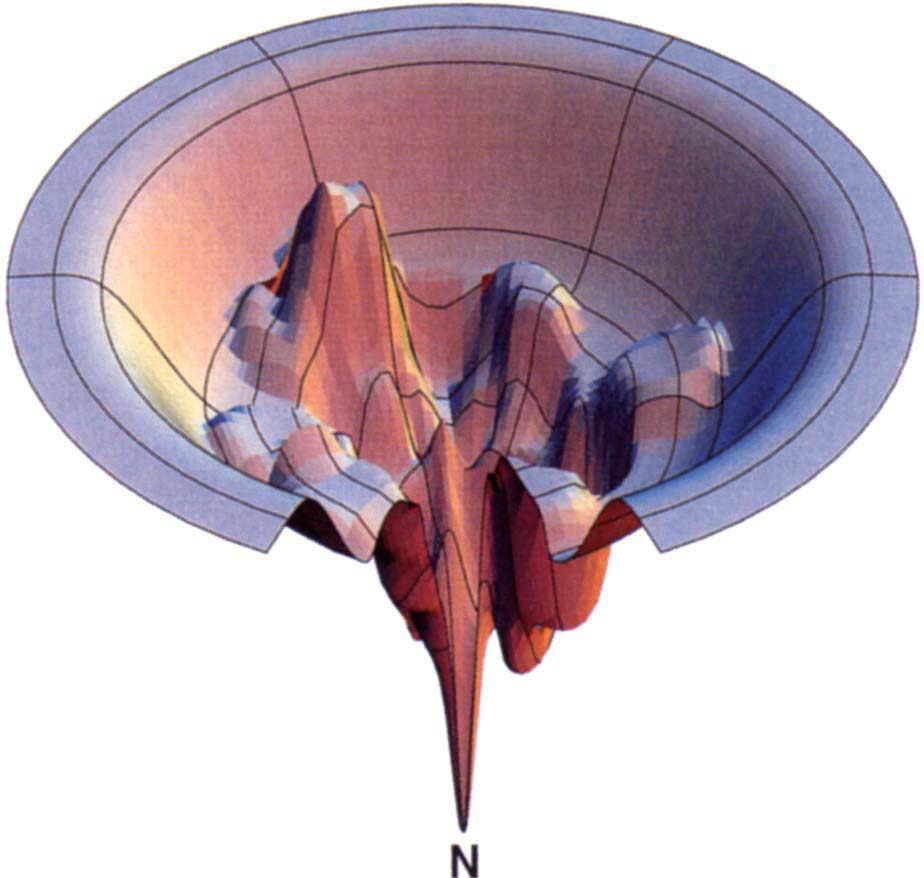
\includegraphics[width=2in]{figures/schematic/dill97-fig4}%
    \label{fig:folding:landscape}}
  \caption{\protect\subref{fig:folding:pathway} A ``double T'' example
    of the pathway model of protein folding, in which the protein
    proceeds from the native state $N$ to the unfolded state $U$ via a
    series of metastable transition states $I_1$ and $I_2$ with two
    ``dead end'' states $I_1^X$ and $I_2^X$.  Adapted from
    \citet{bedard08}.
    \protect\subref{fig:folding:landscape} The landscape model of
    protein folding, in which the protein diffuses through a
    multi-dimensional free energy landscape.  Separate folding
    attempts may take many distinct routes through this landscape on
    the way to the folded state.  Reproduced from
    \citet{dill97}.\label{fig:folding}}
  \end{center}
\end{figure}

When the choice of theoretical approach becomes murky, you must gather
experimental data to help distinguish between similar models.
Separating the pathway model from the funnel model is only marginally
within the realm of current experimental techniques, but with higher
throughput and increased automation it should be easier to make such
distinctions in the near future.


\section{Why \emph{single} molecule?}
\label{sec:single-molecule}

The large size of proteins relative to simpler molecules limits the
information attainable from bulk measurements, because the
macromolecules in a population can have diverse conformations and
behaviors.  Bulk measurements average over these differences,
producing excellent statistics for the mean, but making it difficult
to understand the variation.  The individualized, and sometimes rare,
behaviors of macromolecules can have important implications for their
functions inside the cell.  Single molecule techniques, in which the
macromolecules are studied one at a time, allow direct access to the
variation within the population without averaging.  This provides
important and complementary information about the functional
mechanisms of several biological systems\citep{bustamante08}.

Single molecule techniques provide an opportunity to study protein
folding and unfolding at the level of a single molecule, where the
distinction between the pathway model and funnel model is clearer.
They also provide a convenient benchmark for verifying molecular
dynamics simulations, because it takes lots of computing power to
simulate even one biopolymer with anything close to atomic resolution
over experimental time scales.  Even with significant computing
resources, comparing molecular dynamics results with experimental data
remains elusive.  For example, experimental pulling speeds are on the
order of \bareU{$\mu$m/s}, while simulation pulling speeds are on the
order of \bareU{m/s}\citep{lu98,lu99,rief02,zhao06,berkemeier11}.

% why AFM & what an AFM is
Single molecule techniques for manipulating biopolymers include
optical measurements, \ie, single molecule fluorescence microscopy and
spectroscopy, and mechanical manipulations of individual
macromolecules, \ie, force microscopy and spectroscopy using atomic
force microscopes (AFMs), laser tweezers\citep{kellermayer97,forde02},
magnetic tweezers\citep{smith92}, biomembrane force
probes\citep{merkel99}, and centrifugal
microscopes\citep{halvorsen09}.  These techniques cover a wide range
of approaches, and even when the basic approach is the same
(e.g.\ force microscopy), the different techniques span orders of
magnitude in the range of their controllable parameters.
%
\nomenclature[text ]{AFM}{Atomic force microscope (or microscopy).}

\section{Why \emph{un}folding?}
\label{sec:unfolding}

There's a lot of talk about protein \emph{folding} in this chapter,
while the rest of the thesis (and the title) are about
\emph{unfolding}.  If you understand protein folding, you can use your
understanding to design drugs with a particular conformation, or
predict the conformation of a biologically important receptor
(\cref{sec:folding-problem}).  Understanding protein unfolding is less
directly useful, because unfolded proteins are rarely biologically
relevant (although it does happen\citep{dyson05}).

The focus on unfolding is mainly because it's easier to unravel
proteins by pulling on their ends (\cref{sec:procedure}) than it is to
fold them into their native state by pushing on those ends
(\cref{fig:ligand-receptor,fig:I27}).  For proteins with smooth enough
energy landscapes, the folding and unfolding routes will be similar,
so knowledge about the unfolding behavior \emph{does} shed light on
the folding behavior.

Practically, the distinction between folding and unfolding makes
little difference, because drug designers and doctors are not
consuming SMFS results directly.  For researchers calibrating
molecular dynamics simulations, it doesn't matter if you compare
simulated folding experiments with experimental folding experiments,
or simulated unfolding experiments with experimental unfolding
experiments.  The important thing is to compare your simulation
against \emph{some} experimental benchmarks.  If your molecular
dynamics simulation successfully predicts a protein's unfolding
behavior, it makes me more confident that it will correctly predict
the protein's native folding behavior.


\section{Thesis outline}
\label{sec:outline}

\Cref{sec:methods} of this thesis outlines the apparatus and methods
for single molecule force spectroscopy with an atomic force
microscope.  \Cref{sec:sawsim} presents my \sawsim\ Monte Carlo
simulation for modeling unfolding/refolding behavior.  By comparing
model simulations with experimental measurements, we can gain insight
into the protein's kinetics.  After \cref{sec:sawsim}, you should have
a pretty firm grasp of the underlying physics, so we'll move on to
\cref{sec:pyafm} and discuss my \pyafm\ and \unfoldprotein\ experiment
control software.  With both the kinetic theory and procedure taken
care of, \cref{sec:calibcant} discusses thermal cantilever
calibration, deriving the theoretical approach and presenting my
\calibcant\ automatic calibration software.

Moving away from experiment control, \cref{sec:hooke} presents the
\Hooke\ suite for extracting unfolding force histograms (for
comparison with \sawsim\ simulations).  In \cref{sec:salt}, I pull all
the pieces together (experiment control, post processing, and
simulation) to carry out unfolding experiments on the
immunoglobulin-like domain 27 from human Titin (I27) in buffers with
different ionic strength.  We close with \cref{sec:future}, which
summarizes my conclusions and discusses possible directions for future
work.

%\chapter{Introduction}
\label{sec:intro}

Single molecule force spectroscopy (SMFS) is the study of folding and
unfolding transitions in proteins under tension.  By measuring these
transitions, we hope to gain insight into fundamental protein
behavior.  SMFS is an attempt to bridge the gap between chemists
studying folding and unfolding kinetics in bulk solutions and
theorists simulating protein behavior at the amino-acid level.  An
increased understanding of protein folding would guide researchers in
developing drugs targeting biologically significant receptors and
enzymes.  In this chapter, I describe the protein folding problem in a
general sense (\cref{sec:folding-problem}), discuss theoretical
frameworks for understanding protein folding
(\cref{sec:energy-landscape}), highlight the role of SMFS in extending
this understanding (\cref{sec:single-molecule}), and explain the role
of unfolding experiments in understanding protein folding
(\cref{sec:unfolding}).  The last section in this chapter gives a
roadmap for the rest of the thesis (\cref{sec:outline}).

\section{The protein folding problem}
\label{sec:folding-problem}

% Why study protein folding?
In biological systems the most important molecules, such as proteins,
nucleic acids, and polysaccharides, are all polymers.  Understanding
the properties and functions of these polymeric molecules is crucial
in understanding the molecular mechanisms behind structures and
processes in cells.

% What do genes do?  Why is protein folding interesting?
An organism's genetic code is stored in DNA in the cell nucleus.
DNA sequencing is a fairly well developed field, with fundamental work
such as the Human Genome Project seeing major development in the early
2000s\citep{wolfsberg01,mcpherson01,collins03}.  It is estimated that
human genetic information contains approximately 25,000 genes, each
encoding a protein\citep{claverie01,venter01}.  Knowing the amino acid
sequence for a particular protein, however, does not immediately shed
light on the protein's role in the body, or even the protein's
probable conformation.  Indeed, a protein's conformation is often
vitally important in executing its biological tasks
(\cref{fig:ligand-receptor}).  Unfortunately predicting a protein's
stable conformations from it's amino acid sequence has proven to be
remarkably difficult, as has the inverse problem of finding sequences
that form a given conformation.
%
\nomenclature[text ]{DNA}{Deoxyribonucleic acid.}

\begin{figure}
  \begin{center}
  \includegraphics[width=2in]{figures/biotin-streptavidin/1SWE}%
  \caption{Complex of biotin\index{biotin} (red) and a
    streptavidin\index{streptavidin} tetramer (green)
    (\href{http://dx.doi.org/10.2210/pdb1swe/pdb}{PDB ID: 1SWE})%
    \citep{freitag97}.  The correct streptavidin conformation creates
    the biotin-specific binding pockets.  Biotin-streptavidin is a
    model ligand-receptor pair isolated from the bacterium
    \species{Streptomyces avidinii}%
    \index{Streptomyces@\species{Streptomyces avidnii}}.  Streptavidin
    binds to cell surfaces, and bound biotin increases streptavidin's
    cell-binding affinity\citep{alon90}.  Figure generated with
    \citetalias{pymol}.
    \label{fig:ligand-receptor}}
  \end{center}
\end{figure}


\section{Protein folding energy landscapes}
\label{sec:energy-landscape}

% the free energy landscape
Finding a protein's lowest energy state via a brute force sampling of
all possible conformations is impossibly inefficient, due to the
exponential scaling of possible conformations with protein length, as
outlined by \citet{levinthal69}.  This has lead to a succession of
models explaining the folding mechanism.  For a number of years, the
``pathway'' model of protein folding enjoyed popularity
(\cref{fig:folding:pathway})\citep{levinthal69}.  More recently, the
``landscape'' or ``funnel'' model has come to the fore
(\cref{fig:folding:landscape})\citep{dill97}.  Both of these models
reduce the conformation space to a more approachable analog, and their
success depends on striking a useful balance between simplicity and
accuracy.

\begin{figure}
  \begin{center}
  \subfloat[][]{
    \begin{tikzpicture}[->,node distance=1.5cm]
      \tikzstyle{every state}=[draw=white]
      \node[state] (U)                 {$U$};
      \node[state] (I1)  [right of=U]  {$I_1$};
      \node[state] (I1X) [below of=I1] {$I_1^X$};
      \node[state] (I2)  [right of=I1] {$I_2$};
      \node[state] (I2X) [below of=I2] {$I_2^X$};
      \node[state] (N)   [right of=I2] {$N$};
    
      \path[<->] (U)  edge (I1)
                 (I1) edge (I1X)
                 (I1) edge (I2)
                 (I2) edge (I2X)
                 (I2) edge (N);
    \end{tikzpicture}\label{fig:folding:pathway}}
  % \hspace{.25in}%
  \subfloat[][]{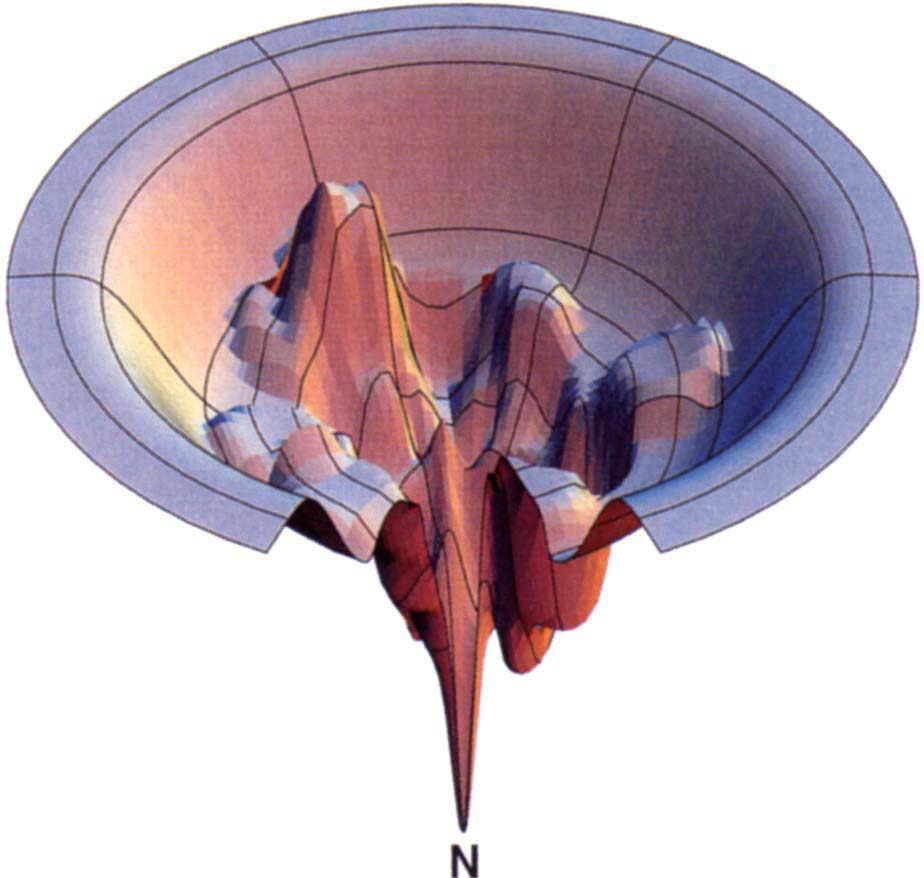
\includegraphics[width=2in]{figures/schematic/dill97-fig4}%
    \label{fig:folding:landscape}}
  \caption{\protect\subref{fig:folding:pathway} A ``double T'' example
    of the pathway model of protein folding, in which the protein
    proceeds from the native state $N$ to the unfolded state $U$ via a
    series of metastable transition states $I_1$ and $I_2$ with two
    ``dead end'' states $I_1^X$ and $I_2^X$.  Adapted from
    \citet{bedard08}.
    \protect\subref{fig:folding:landscape} The landscape model of
    protein folding, in which the protein diffuses through a
    multi-dimensional free energy landscape.  Separate folding
    attempts may take many distinct routes through this landscape on
    the way to the folded state.  Reproduced from
    \citet{dill97}.\label{fig:folding}}
  \end{center}
\end{figure}

When the choice of theoretical approach becomes murky, you must gather
experimental data to help distinguish between similar models.
Separating the pathway model from the funnel model is only marginally
within the realm of current experimental techniques, but with higher
throughput and increased automation it should be easier to make such
distinctions in the near future.


\section{Why \emph{single} molecule?}
\label{sec:single-molecule}

The large size of proteins relative to simpler molecules limits the
information attainable from bulk measurements, because the
macromolecules in a population can have diverse conformations and
behaviors.  Bulk measurements average over these differences,
producing excellent statistics for the mean, but making it difficult
to understand the variation.  The individualized, and sometimes rare,
behaviors of macromolecules can have important implications for their
functions inside the cell.  Single molecule techniques, in which the
macromolecules are studied one at a time, allow direct access to the
variation within the population without averaging.  This provides
important and complementary information about the functional
mechanisms of several biological systems\citep{bustamante08}.

Single molecule techniques provide an opportunity to study protein
folding and unfolding at the level of a single molecule, where the
distinction between the pathway model and funnel model is clearer.
They also provide a convenient benchmark for verifying molecular
dynamics simulations, because it takes lots of computing power to
simulate even one biopolymer with anything close to atomic resolution
over experimental time scales.  Even with significant computing
resources, comparing molecular dynamics results with experimental data
remains elusive.  For example, experimental pulling speeds are on the
order of \bareU{$\mu$m/s}, while simulation pulling speeds are on the
order of \bareU{m/s}\citep{lu98,lu99,rief02,zhao06,berkemeier11}.

% why AFM & what an AFM is
Single molecule techniques for manipulating biopolymers include
optical measurements, \ie, single molecule fluorescence microscopy and
spectroscopy, and mechanical manipulations of individual
macromolecules, \ie, force microscopy and spectroscopy using atomic
force microscopes (AFMs), laser tweezers\citep{kellermayer97,forde02},
magnetic tweezers\citep{smith92}, biomembrane force
probes\citep{merkel99}, and centrifugal
microscopes\citep{halvorsen09}.  These techniques cover a wide range
of approaches, and even when the basic approach is the same
(e.g.\ force microscopy), the different techniques span orders of
magnitude in the range of their controllable parameters.
%
\nomenclature[text ]{AFM}{Atomic force microscope (or microscopy).}

\section{Why \emph{un}folding?}
\label{sec:unfolding}

There's a lot of talk about protein \emph{folding} in this chapter,
while the rest of the thesis (and the title) are about
\emph{unfolding}.  If you understand protein folding, you can use your
understanding to design drugs with a particular conformation, or
predict the conformation of a biologically important receptor
(\cref{sec:folding-problem}).  Understanding protein unfolding is less
directly useful, because unfolded proteins are rarely biologically
relevant (although it does happen\citep{dyson05}).

The focus on unfolding is mainly because it's easier to unravel
proteins by pulling on their ends (\cref{sec:procedure}) than it is to
fold them into their native state by pushing on those ends
(\cref{fig:ligand-receptor,fig:I27}).  For proteins with smooth enough
energy landscapes, the folding and unfolding routes will be similar,
so knowledge about the unfolding behavior \emph{does} shed light on
the folding behavior.

Practically, the distinction between folding and unfolding makes
little difference, because drug designers and doctors are not
consuming SMFS results directly.  For researchers calibrating
molecular dynamics simulations, it doesn't matter if you compare
simulated folding experiments with experimental folding experiments,
or simulated unfolding experiments with experimental unfolding
experiments.  The important thing is to compare your simulation
against \emph{some} experimental benchmarks.  If your molecular
dynamics simulation successfully predicts a protein's unfolding
behavior, it makes me more confident that it will correctly predict
the protein's native folding behavior.


\section{Thesis outline}
\label{sec:outline}

\Cref{sec:methods} of this thesis outlines the apparatus and methods
for single molecule force spectroscopy with an atomic force
microscope.  \Cref{sec:sawsim} presents my \sawsim\ Monte Carlo
simulation for modeling unfolding/refolding behavior.  By comparing
model simulations with experimental measurements, we can gain insight
into the protein's kinetics.  After \cref{sec:sawsim}, you should have
a pretty firm grasp of the underlying physics, so we'll move on to
\cref{sec:pyafm} and discuss my \pyafm\ and \unfoldprotein\ experiment
control software.  With both the kinetic theory and procedure taken
care of, \cref{sec:calibcant} discusses thermal cantilever
calibration, deriving the theoretical approach and presenting my
\calibcant\ automatic calibration software.

Moving away from experiment control, \cref{sec:hooke} presents the
\Hooke\ suite for extracting unfolding force histograms (for
comparison with \sawsim\ simulations).  In \cref{sec:salt}, I pull all
the pieces together (experiment control, post processing, and
simulation) to carry out unfolding experiments on the
immunoglobulin-like domain 27 from human Titin (I27) in buffers with
different ionic strength.  We close with \cref{sec:future}, which
summarizes my conclusions and discusses possible directions for future
work.

\chapter{Introduction}
\label{sec:intro}

Single molecule force spectroscopy (SMFS) is the study of folding and
unfolding transitions in proteins under tension.  By measuring these
transitions, we hope to gain insight into fundamental protein
behavior.  SMFS is an attempt to bridge the gap between chemists
studying folding and unfolding kinetics in bulk solutions and
theorists simulating protein behavior at the amino-acid level.  An
increased understanding of protein folding would guide researchers in
developing drugs targeting biologically significant receptors and
enzymes.  In this chapter, I describe the protein folding problem in a
general sense (\cref{sec:folding-problem}), discuss theoretical
frameworks for understanding protein folding
(\cref{sec:energy-landscape}), highlight the role of SMFS in extending
this understanding (\cref{sec:single-molecule}), and explain the role
of unfolding experiments in understanding protein folding
(\cref{sec:unfolding}).  The last section in this chapter gives a
roadmap for the rest of the thesis (\cref{sec:outline}).

\section{The protein folding problem}
\label{sec:folding-problem}

% Why study protein folding?
In biological systems the most important molecules, such as proteins,
nucleic acids, and polysaccharides, are all polymers.  Understanding
the properties and functions of these polymeric molecules is crucial
in understanding the molecular mechanisms behind structures and
processes in cells.

% What do genes do?  Why is protein folding interesting?
An organism's genetic code is stored in DNA in the cell nucleus.
DNA sequencing is a fairly well developed field, with fundamental work
such as the Human Genome Project seeing major development in the early
2000s\citep{wolfsberg01,mcpherson01,collins03}.  It is estimated that
human genetic information contains approximately 25,000 genes, each
encoding a protein\citep{claverie01,venter01}.  Knowing the amino acid
sequence for a particular protein, however, does not immediately shed
light on the protein's role in the body, or even the protein's
probable conformation.  Indeed, a protein's conformation is often
vitally important in executing its biological tasks
(\cref{fig:ligand-receptor}).  Unfortunately predicting a protein's
stable conformations from it's amino acid sequence has proven to be
remarkably difficult, as has the inverse problem of finding sequences
that form a given conformation.
%
\nomenclature[text ]{DNA}{Deoxyribonucleic acid.}

\begin{figure}
  \begin{center}
  \includegraphics[width=2in]{figures/biotin-streptavidin/1SWE}%
  \caption{Complex of biotin\index{biotin} (red) and a
    streptavidin\index{streptavidin} tetramer (green)
    (\href{http://dx.doi.org/10.2210/pdb1swe/pdb}{PDB ID: 1SWE})%
    \citep{freitag97}.  The correct streptavidin conformation creates
    the biotin-specific binding pockets.  Biotin-streptavidin is a
    model ligand-receptor pair isolated from the bacterium
    \species{Streptomyces avidinii}%
    \index{Streptomyces@\species{Streptomyces avidnii}}.  Streptavidin
    binds to cell surfaces, and bound biotin increases streptavidin's
    cell-binding affinity\citep{alon90}.  Figure generated with
    \citetalias{pymol}.
    \label{fig:ligand-receptor}}
  \end{center}
\end{figure}


\section{Protein folding energy landscapes}
\label{sec:energy-landscape}

% the free energy landscape
Finding a protein's lowest energy state via a brute force sampling of
all possible conformations is impossibly inefficient, due to the
exponential scaling of possible conformations with protein length, as
outlined by \citet{levinthal69}.  This has lead to a succession of
models explaining the folding mechanism.  For a number of years, the
``pathway'' model of protein folding enjoyed popularity
(\cref{fig:folding:pathway})\citep{levinthal69}.  More recently, the
``landscape'' or ``funnel'' model has come to the fore
(\cref{fig:folding:landscape})\citep{dill97}.  Both of these models
reduce the conformation space to a more approachable analog, and their
success depends on striking a useful balance between simplicity and
accuracy.

\begin{figure}
  \begin{center}
  \subfloat[][]{
    \begin{tikzpicture}[->,node distance=1.5cm]
      \tikzstyle{every state}=[draw=white]
      \node[state] (U)                 {$U$};
      \node[state] (I1)  [right of=U]  {$I_1$};
      \node[state] (I1X) [below of=I1] {$I_1^X$};
      \node[state] (I2)  [right of=I1] {$I_2$};
      \node[state] (I2X) [below of=I2] {$I_2^X$};
      \node[state] (N)   [right of=I2] {$N$};
    
      \path[<->] (U)  edge (I1)
                 (I1) edge (I1X)
                 (I1) edge (I2)
                 (I2) edge (I2X)
                 (I2) edge (N);
    \end{tikzpicture}\label{fig:folding:pathway}}
  % \hspace{.25in}%
  \subfloat[][]{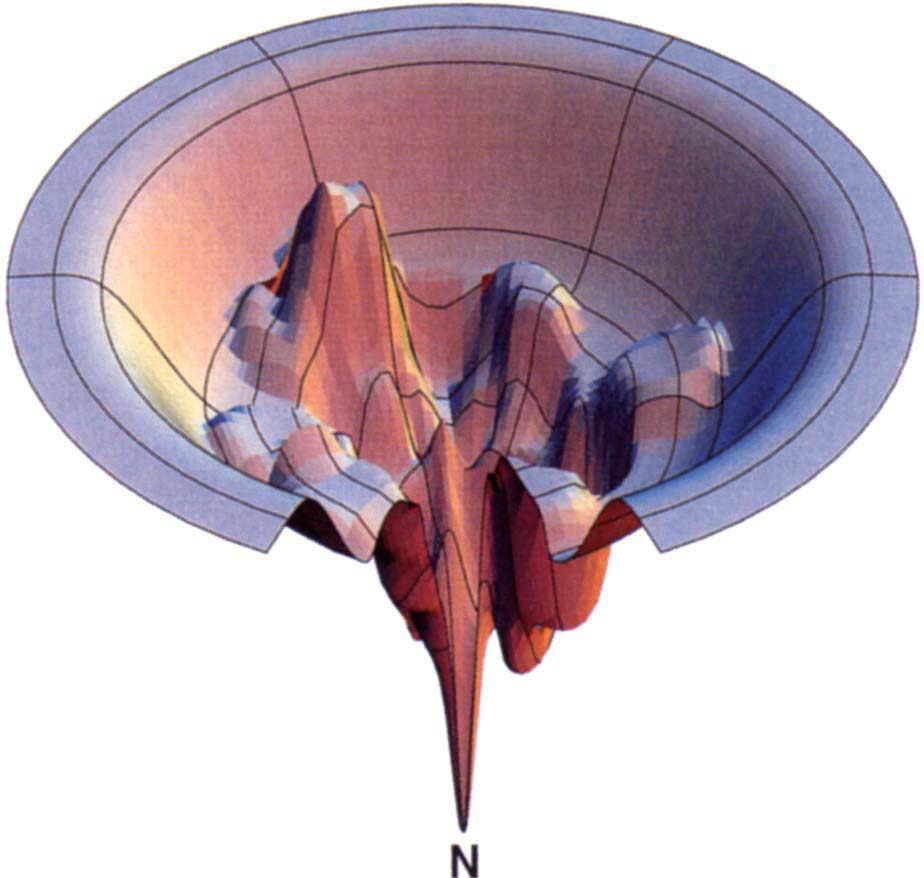
\includegraphics[width=2in]{figures/schematic/dill97-fig4}%
    \label{fig:folding:landscape}}
  \caption{\protect\subref{fig:folding:pathway} A ``double T'' example
    of the pathway model of protein folding, in which the protein
    proceeds from the native state $N$ to the unfolded state $U$ via a
    series of metastable transition states $I_1$ and $I_2$ with two
    ``dead end'' states $I_1^X$ and $I_2^X$.  Adapted from
    \citet{bedard08}.
    \protect\subref{fig:folding:landscape} The landscape model of
    protein folding, in which the protein diffuses through a
    multi-dimensional free energy landscape.  Separate folding
    attempts may take many distinct routes through this landscape on
    the way to the folded state.  Reproduced from
    \citet{dill97}.\label{fig:folding}}
  \end{center}
\end{figure}

When the choice of theoretical approach becomes murky, you must gather
experimental data to help distinguish between similar models.
Separating the pathway model from the funnel model is only marginally
within the realm of current experimental techniques, but with higher
throughput and increased automation it should be easier to make such
distinctions in the near future.


\section{Why \emph{single} molecule?}
\label{sec:single-molecule}

The large size of proteins relative to simpler molecules limits the
information attainable from bulk measurements, because the
macromolecules in a population can have diverse conformations and
behaviors.  Bulk measurements average over these differences,
producing excellent statistics for the mean, but making it difficult
to understand the variation.  The individualized, and sometimes rare,
behaviors of macromolecules can have important implications for their
functions inside the cell.  Single molecule techniques, in which the
macromolecules are studied one at a time, allow direct access to the
variation within the population without averaging.  This provides
important and complementary information about the functional
mechanisms of several biological systems\citep{bustamante08}.

Single molecule techniques provide an opportunity to study protein
folding and unfolding at the level of a single molecule, where the
distinction between the pathway model and funnel model is clearer.
They also provide a convenient benchmark for verifying molecular
dynamics simulations, because it takes lots of computing power to
simulate even one biopolymer with anything close to atomic resolution
over experimental time scales.  Even with significant computing
resources, comparing molecular dynamics results with experimental data
remains elusive.  For example, experimental pulling speeds are on the
order of \bareU{$\mu$m/s}, while simulation pulling speeds are on the
order of \bareU{m/s}\citep{lu98,lu99,rief02,zhao06,berkemeier11}.

% why AFM & what an AFM is
Single molecule techniques for manipulating biopolymers include
optical measurements, \ie, single molecule fluorescence microscopy and
spectroscopy, and mechanical manipulations of individual
macromolecules, \ie, force microscopy and spectroscopy using atomic
force microscopes (AFMs), laser tweezers\citep{kellermayer97,forde02},
magnetic tweezers\citep{smith92}, biomembrane force
probes\citep{merkel99}, and centrifugal
microscopes\citep{halvorsen09}.  These techniques cover a wide range
of approaches, and even when the basic approach is the same
(e.g.\ force microscopy), the different techniques span orders of
magnitude in the range of their controllable parameters.
%
\nomenclature[text ]{AFM}{Atomic force microscope (or microscopy).}

\section{Why \emph{un}folding?}
\label{sec:unfolding}

There's a lot of talk about protein \emph{folding} in this chapter,
while the rest of the thesis (and the title) are about
\emph{unfolding}.  If you understand protein folding, you can use your
understanding to design drugs with a particular conformation, or
predict the conformation of a biologically important receptor
(\cref{sec:folding-problem}).  Understanding protein unfolding is less
directly useful, because unfolded proteins are rarely biologically
relevant (although it does happen\citep{dyson05}).

The focus on unfolding is mainly because it's easier to unravel
proteins by pulling on their ends (\cref{sec:procedure}) than it is to
fold them into their native state by pushing on those ends
(\cref{fig:ligand-receptor,fig:I27}).  For proteins with smooth enough
energy landscapes, the folding and unfolding routes will be similar,
so knowledge about the unfolding behavior \emph{does} shed light on
the folding behavior.

Practically, the distinction between folding and unfolding makes
little difference, because drug designers and doctors are not
consuming SMFS results directly.  For researchers calibrating
molecular dynamics simulations, it doesn't matter if you compare
simulated folding experiments with experimental folding experiments,
or simulated unfolding experiments with experimental unfolding
experiments.  The important thing is to compare your simulation
against \emph{some} experimental benchmarks.  If your molecular
dynamics simulation successfully predicts a protein's unfolding
behavior, it makes me more confident that it will correctly predict
the protein's native folding behavior.


\section{Thesis outline}
\label{sec:outline}

\Cref{sec:methods} of this thesis outlines the apparatus and methods
for single molecule force spectroscopy with an atomic force
microscope.  \Cref{sec:sawsim} presents my \sawsim\ Monte Carlo
simulation for modeling unfolding/refolding behavior.  By comparing
model simulations with experimental measurements, we can gain insight
into the protein's kinetics.  After \cref{sec:sawsim}, you should have
a pretty firm grasp of the underlying physics, so we'll move on to
\cref{sec:pyafm} and discuss my \pyafm\ and \unfoldprotein\ experiment
control software.  With both the kinetic theory and procedure taken
care of, \cref{sec:calibcant} discusses thermal cantilever
calibration, deriving the theoretical approach and presenting my
\calibcant\ automatic calibration software.

Moving away from experiment control, \cref{sec:hooke} presents the
\Hooke\ suite for extracting unfolding force histograms (for
comparison with \sawsim\ simulations).  In \cref{sec:salt}, I pull all
the pieces together (experiment control, post processing, and
simulation) to carry out unfolding experiments on the
immunoglobulin-like domain 27 from human Titin (I27) in buffers with
different ionic strength.  We close with \cref{sec:future}, which
summarizes my conclusions and discusses possible directions for future
work.

\chapter{Introduction}
\label{sec:intro}

Single molecule force spectroscopy (SMFS) is the study of folding and
unfolding transitions in proteins under tension.  By measuring these
transitions, we hope to gain insight into fundamental protein
behavior.  SMFS is an attempt to bridge the gap between chemists
studying folding and unfolding kinetics in bulk solutions and
theorists simulating protein behavior at the amino-acid level.  An
increased understanding of protein folding would guide researchers in
developing drugs targeting biologically significant receptors and
enzymes.  In this chapter, I describe the protein folding problem in a
general sense (\cref{sec:folding-problem}), discuss theoretical
frameworks for understanding protein folding
(\cref{sec:energy-landscape}), highlight the role of SMFS in extending
this understanding (\cref{sec:single-molecule}), and explain the role
of unfolding experiments in understanding protein folding
(\cref{sec:unfolding}).  The last section in this chapter gives a
roadmap for the rest of the thesis (\cref{sec:outline}).

\section{The protein folding problem}
\label{sec:folding-problem}

% Why study protein folding?
In biological systems the most important molecules, such as proteins,
nucleic acids, and polysaccharides, are all polymers.  Understanding
the properties and functions of these polymeric molecules is crucial
in understanding the molecular mechanisms behind structures and
processes in cells.

% What do genes do?  Why is protein folding interesting?
An organism's genetic code is stored in DNA in the cell nucleus.
DNA sequencing is a fairly well developed field, with fundamental work
such as the Human Genome Project seeing major development in the early
2000s\citep{wolfsberg01,mcpherson01,collins03}.  It is estimated that
human genetic information contains approximately 25,000 genes, each
encoding a protein\citep{claverie01,venter01}.  Knowing the amino acid
sequence for a particular protein, however, does not immediately shed
light on the protein's role in the body, or even the protein's
probable conformation.  Indeed, a protein's conformation is often
vitally important in executing its biological tasks
(\cref{fig:ligand-receptor}).  Unfortunately predicting a protein's
stable conformations from it's amino acid sequence has proven to be
remarkably difficult, as has the inverse problem of finding sequences
that form a given conformation.
%
\nomenclature[text ]{DNA}{Deoxyribonucleic acid.}

\begin{figure}
  \begin{center}
  \includegraphics[width=2in]{figures/biotin-streptavidin/1SWE}%
  \caption{Complex of biotin\index{biotin} (red) and a
    streptavidin\index{streptavidin} tetramer (green)
    (\href{http://dx.doi.org/10.2210/pdb1swe/pdb}{PDB ID: 1SWE})%
    \citep{freitag97}.  The correct streptavidin conformation creates
    the biotin-specific binding pockets.  Biotin-streptavidin is a
    model ligand-receptor pair isolated from the bacterium
    \species{Streptomyces avidinii}%
    \index{Streptomyces@\species{Streptomyces avidnii}}.  Streptavidin
    binds to cell surfaces, and bound biotin increases streptavidin's
    cell-binding affinity\citep{alon90}.  Figure generated with
    \citetalias{pymol}.
    \label{fig:ligand-receptor}}
  \end{center}
\end{figure}


\section{Protein folding energy landscapes}
\label{sec:energy-landscape}

% the free energy landscape
Finding a protein's lowest energy state via a brute force sampling of
all possible conformations is impossibly inefficient, due to the
exponential scaling of possible conformations with protein length, as
outlined by \citet{levinthal69}.  This has lead to a succession of
models explaining the folding mechanism.  For a number of years, the
``pathway'' model of protein folding enjoyed popularity
(\cref{fig:folding:pathway})\citep{levinthal69}.  More recently, the
``landscape'' or ``funnel'' model has come to the fore
(\cref{fig:folding:landscape})\citep{dill97}.  Both of these models
reduce the conformation space to a more approachable analog, and their
success depends on striking a useful balance between simplicity and
accuracy.

\begin{figure}
  \begin{center}
  \subfloat[][]{
    \begin{tikzpicture}[->,node distance=1.5cm]
      \tikzstyle{every state}=[draw=white]
      \node[state] (U)                 {$U$};
      \node[state] (I1)  [right of=U]  {$I_1$};
      \node[state] (I1X) [below of=I1] {$I_1^X$};
      \node[state] (I2)  [right of=I1] {$I_2$};
      \node[state] (I2X) [below of=I2] {$I_2^X$};
      \node[state] (N)   [right of=I2] {$N$};
    
      \path[<->] (U)  edge (I1)
                 (I1) edge (I1X)
                 (I1) edge (I2)
                 (I2) edge (I2X)
                 (I2) edge (N);
    \end{tikzpicture}\label{fig:folding:pathway}}
  % \hspace{.25in}%
  \subfloat[][]{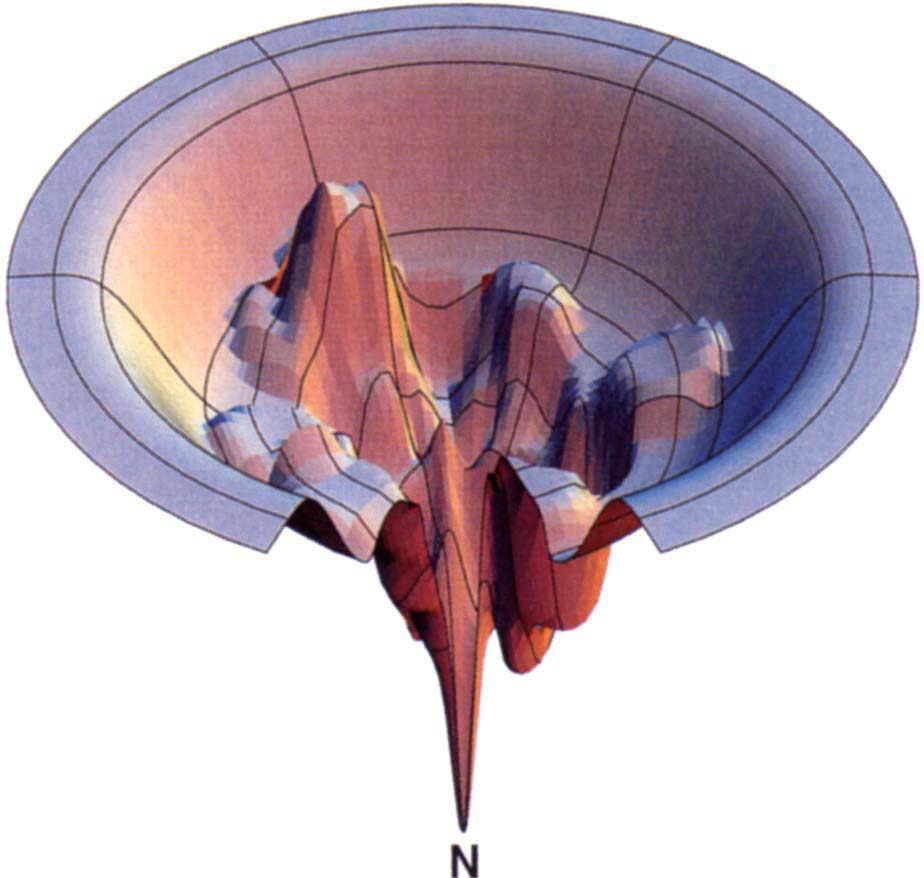
\includegraphics[width=2in]{figures/schematic/dill97-fig4}%
    \label{fig:folding:landscape}}
  \caption{\protect\subref{fig:folding:pathway} A ``double T'' example
    of the pathway model of protein folding, in which the protein
    proceeds from the native state $N$ to the unfolded state $U$ via a
    series of metastable transition states $I_1$ and $I_2$ with two
    ``dead end'' states $I_1^X$ and $I_2^X$.  Adapted from
    \citet{bedard08}.
    \protect\subref{fig:folding:landscape} The landscape model of
    protein folding, in which the protein diffuses through a
    multi-dimensional free energy landscape.  Separate folding
    attempts may take many distinct routes through this landscape on
    the way to the folded state.  Reproduced from
    \citet{dill97}.\label{fig:folding}}
  \end{center}
\end{figure}

When the choice of theoretical approach becomes murky, you must gather
experimental data to help distinguish between similar models.
Separating the pathway model from the funnel model is only marginally
within the realm of current experimental techniques, but with higher
throughput and increased automation it should be easier to make such
distinctions in the near future.


\section{Why \emph{single} molecule?}
\label{sec:single-molecule}

The large size of proteins relative to simpler molecules limits the
information attainable from bulk measurements, because the
macromolecules in a population can have diverse conformations and
behaviors.  Bulk measurements average over these differences,
producing excellent statistics for the mean, but making it difficult
to understand the variation.  The individualized, and sometimes rare,
behaviors of macromolecules can have important implications for their
functions inside the cell.  Single molecule techniques, in which the
macromolecules are studied one at a time, allow direct access to the
variation within the population without averaging.  This provides
important and complementary information about the functional
mechanisms of several biological systems\citep{bustamante08}.

Single molecule techniques provide an opportunity to study protein
folding and unfolding at the level of a single molecule, where the
distinction between the pathway model and funnel model is clearer.
They also provide a convenient benchmark for verifying molecular
dynamics simulations, because it takes lots of computing power to
simulate even one biopolymer with anything close to atomic resolution
over experimental time scales.  Even with significant computing
resources, comparing molecular dynamics results with experimental data
remains elusive.  For example, experimental pulling speeds are on the
order of \bareU{$\mu$m/s}, while simulation pulling speeds are on the
order of \bareU{m/s}\citep{lu98,lu99,rief02,zhao06,berkemeier11}.

% why AFM & what an AFM is
Single molecule techniques for manipulating biopolymers include
optical measurements, \ie, single molecule fluorescence microscopy and
spectroscopy, and mechanical manipulations of individual
macromolecules, \ie, force microscopy and spectroscopy using atomic
force microscopes (AFMs), laser tweezers\citep{kellermayer97,forde02},
magnetic tweezers\citep{smith92}, biomembrane force
probes\citep{merkel99}, and centrifugal
microscopes\citep{halvorsen09}.  These techniques cover a wide range
of approaches, and even when the basic approach is the same
(e.g.\ force microscopy), the different techniques span orders of
magnitude in the range of their controllable parameters.
%
\nomenclature[text ]{AFM}{Atomic force microscope (or microscopy).}

\section{Why \emph{un}folding?}
\label{sec:unfolding}

There's a lot of talk about protein \emph{folding} in this chapter,
while the rest of the thesis (and the title) are about
\emph{unfolding}.  If you understand protein folding, you can use your
understanding to design drugs with a particular conformation, or
predict the conformation of a biologically important receptor
(\cref{sec:folding-problem}).  Understanding protein unfolding is less
directly useful, because unfolded proteins are rarely biologically
relevant (although it does happen\citep{dyson05}).

The focus on unfolding is mainly because it's easier to unravel
proteins by pulling on their ends (\cref{sec:procedure}) than it is to
fold them into their native state by pushing on those ends
(\cref{fig:ligand-receptor,fig:I27}).  For proteins with smooth enough
energy landscapes, the folding and unfolding routes will be similar,
so knowledge about the unfolding behavior \emph{does} shed light on
the folding behavior.

Practically, the distinction between folding and unfolding makes
little difference, because drug designers and doctors are not
consuming SMFS results directly.  For researchers calibrating
molecular dynamics simulations, it doesn't matter if you compare
simulated folding experiments with experimental folding experiments,
or simulated unfolding experiments with experimental unfolding
experiments.  The important thing is to compare your simulation
against \emph{some} experimental benchmarks.  If your molecular
dynamics simulation successfully predicts a protein's unfolding
behavior, it makes me more confident that it will correctly predict
the protein's native folding behavior.


\section{Thesis outline}
\label{sec:outline}

\Cref{sec:methods} of this thesis outlines the apparatus and methods
for single molecule force spectroscopy with an atomic force
microscope.  \Cref{sec:sawsim} presents my \sawsim\ Monte Carlo
simulation for modeling unfolding/refolding behavior.  By comparing
model simulations with experimental measurements, we can gain insight
into the protein's kinetics.  After \cref{sec:sawsim}, you should have
a pretty firm grasp of the underlying physics, so we'll move on to
\cref{sec:pyafm} and discuss my \pyafm\ and \unfoldprotein\ experiment
control software.  With both the kinetic theory and procedure taken
care of, \cref{sec:calibcant} discusses thermal cantilever
calibration, deriving the theoretical approach and presenting my
\calibcant\ automatic calibration software.

Moving away from experiment control, \cref{sec:hooke} presents the
\Hooke\ suite for extracting unfolding force histograms (for
comparison with \sawsim\ simulations).  In \cref{sec:salt}, I pull all
the pieces together (experiment control, post processing, and
simulation) to carry out unfolding experiments on the
immunoglobulin-like domain 27 from human Titin (I27) in buffers with
different ionic strength.  We close with \cref{sec:future}, which
summarizes my conclusions and discusses possible directions for future
work.

\end{thesis}

\bibliography{%
  blurb/main,%
  apparatus/main,%
%  sawsim/main,% currently empty
  pyafm/main,%
  calibcant/main,%
  hooke/main,%
  salt/main,%
  future/main,%
  packaging/main,%
  figures/main,%
  root}

\appendix
\chapter{Introduction}
\label{sec:intro}

Single molecule force spectroscopy (SMFS) is the study of folding and
unfolding transitions in proteins under tension.  By measuring these
transitions, we hope to gain insight into fundamental protein
behavior.  SMFS is an attempt to bridge the gap between chemists
studying folding and unfolding kinetics in bulk solutions and
theorists simulating protein behavior at the amino-acid level.  An
increased understanding of protein folding would guide researchers in
developing drugs targeting biologically significant receptors and
enzymes.  In this chapter, I describe the protein folding problem in a
general sense (\cref{sec:folding-problem}), discuss theoretical
frameworks for understanding protein folding
(\cref{sec:energy-landscape}), highlight the role of SMFS in extending
this understanding (\cref{sec:single-molecule}), and explain the role
of unfolding experiments in understanding protein folding
(\cref{sec:unfolding}).  The last section in this chapter gives a
roadmap for the rest of the thesis (\cref{sec:outline}).

\section{The protein folding problem}
\label{sec:folding-problem}

% Why study protein folding?
In biological systems the most important molecules, such as proteins,
nucleic acids, and polysaccharides, are all polymers.  Understanding
the properties and functions of these polymeric molecules is crucial
in understanding the molecular mechanisms behind structures and
processes in cells.

% What do genes do?  Why is protein folding interesting?
An organism's genetic code is stored in DNA in the cell nucleus.
DNA sequencing is a fairly well developed field, with fundamental work
such as the Human Genome Project seeing major development in the early
2000s\citep{wolfsberg01,mcpherson01,collins03}.  It is estimated that
human genetic information contains approximately 25,000 genes, each
encoding a protein\citep{claverie01,venter01}.  Knowing the amino acid
sequence for a particular protein, however, does not immediately shed
light on the protein's role in the body, or even the protein's
probable conformation.  Indeed, a protein's conformation is often
vitally important in executing its biological tasks
(\cref{fig:ligand-receptor}).  Unfortunately predicting a protein's
stable conformations from it's amino acid sequence has proven to be
remarkably difficult, as has the inverse problem of finding sequences
that form a given conformation.
%
\nomenclature[text ]{DNA}{Deoxyribonucleic acid.}

\begin{figure}
  \begin{center}
  \includegraphics[width=2in]{figures/biotin-streptavidin/1SWE}%
  \caption{Complex of biotin\index{biotin} (red) and a
    streptavidin\index{streptavidin} tetramer (green)
    (\href{http://dx.doi.org/10.2210/pdb1swe/pdb}{PDB ID: 1SWE})%
    \citep{freitag97}.  The correct streptavidin conformation creates
    the biotin-specific binding pockets.  Biotin-streptavidin is a
    model ligand-receptor pair isolated from the bacterium
    \species{Streptomyces avidinii}%
    \index{Streptomyces@\species{Streptomyces avidnii}}.  Streptavidin
    binds to cell surfaces, and bound biotin increases streptavidin's
    cell-binding affinity\citep{alon90}.  Figure generated with
    \citetalias{pymol}.
    \label{fig:ligand-receptor}}
  \end{center}
\end{figure}


\section{Protein folding energy landscapes}
\label{sec:energy-landscape}

% the free energy landscape
Finding a protein's lowest energy state via a brute force sampling of
all possible conformations is impossibly inefficient, due to the
exponential scaling of possible conformations with protein length, as
outlined by \citet{levinthal69}.  This has lead to a succession of
models explaining the folding mechanism.  For a number of years, the
``pathway'' model of protein folding enjoyed popularity
(\cref{fig:folding:pathway})\citep{levinthal69}.  More recently, the
``landscape'' or ``funnel'' model has come to the fore
(\cref{fig:folding:landscape})\citep{dill97}.  Both of these models
reduce the conformation space to a more approachable analog, and their
success depends on striking a useful balance between simplicity and
accuracy.

\begin{figure}
  \begin{center}
  \subfloat[][]{
    \begin{tikzpicture}[->,node distance=1.5cm]
      \tikzstyle{every state}=[draw=white]
      \node[state] (U)                 {$U$};
      \node[state] (I1)  [right of=U]  {$I_1$};
      \node[state] (I1X) [below of=I1] {$I_1^X$};
      \node[state] (I2)  [right of=I1] {$I_2$};
      \node[state] (I2X) [below of=I2] {$I_2^X$};
      \node[state] (N)   [right of=I2] {$N$};
    
      \path[<->] (U)  edge (I1)
                 (I1) edge (I1X)
                 (I1) edge (I2)
                 (I2) edge (I2X)
                 (I2) edge (N);
    \end{tikzpicture}\label{fig:folding:pathway}}
  % \hspace{.25in}%
  \subfloat[][]{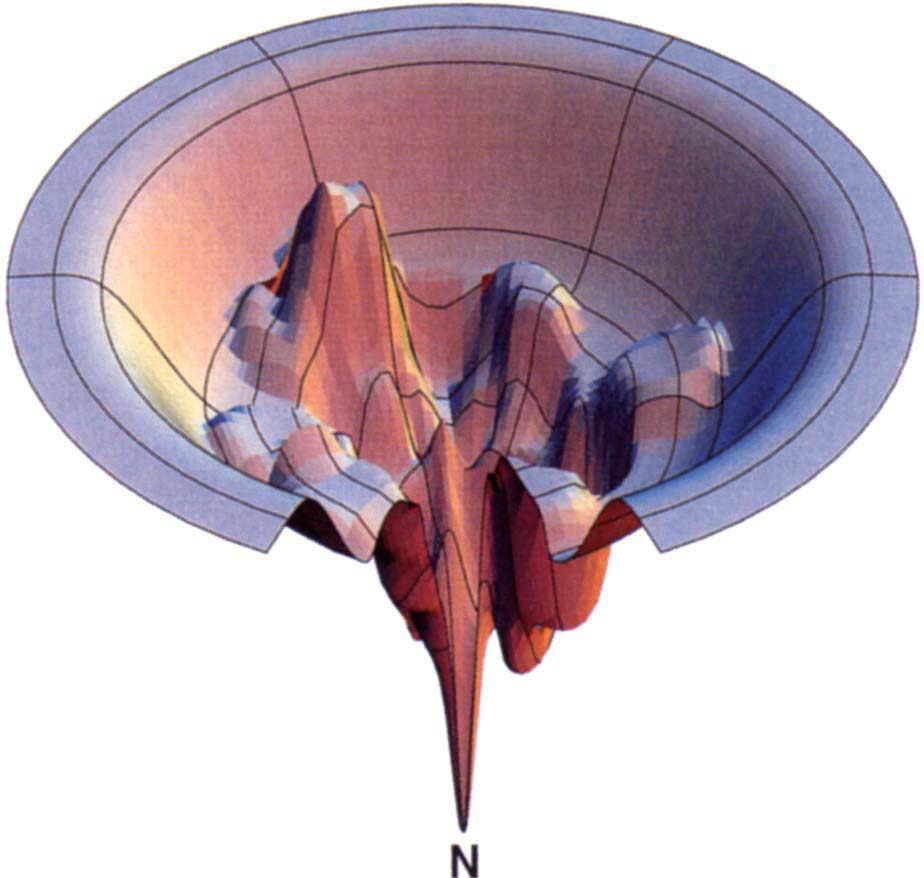
\includegraphics[width=2in]{figures/schematic/dill97-fig4}%
    \label{fig:folding:landscape}}
  \caption{\protect\subref{fig:folding:pathway} A ``double T'' example
    of the pathway model of protein folding, in which the protein
    proceeds from the native state $N$ to the unfolded state $U$ via a
    series of metastable transition states $I_1$ and $I_2$ with two
    ``dead end'' states $I_1^X$ and $I_2^X$.  Adapted from
    \citet{bedard08}.
    \protect\subref{fig:folding:landscape} The landscape model of
    protein folding, in which the protein diffuses through a
    multi-dimensional free energy landscape.  Separate folding
    attempts may take many distinct routes through this landscape on
    the way to the folded state.  Reproduced from
    \citet{dill97}.\label{fig:folding}}
  \end{center}
\end{figure}

When the choice of theoretical approach becomes murky, you must gather
experimental data to help distinguish between similar models.
Separating the pathway model from the funnel model is only marginally
within the realm of current experimental techniques, but with higher
throughput and increased automation it should be easier to make such
distinctions in the near future.


\section{Why \emph{single} molecule?}
\label{sec:single-molecule}

The large size of proteins relative to simpler molecules limits the
information attainable from bulk measurements, because the
macromolecules in a population can have diverse conformations and
behaviors.  Bulk measurements average over these differences,
producing excellent statistics for the mean, but making it difficult
to understand the variation.  The individualized, and sometimes rare,
behaviors of macromolecules can have important implications for their
functions inside the cell.  Single molecule techniques, in which the
macromolecules are studied one at a time, allow direct access to the
variation within the population without averaging.  This provides
important and complementary information about the functional
mechanisms of several biological systems\citep{bustamante08}.

Single molecule techniques provide an opportunity to study protein
folding and unfolding at the level of a single molecule, where the
distinction between the pathway model and funnel model is clearer.
They also provide a convenient benchmark for verifying molecular
dynamics simulations, because it takes lots of computing power to
simulate even one biopolymer with anything close to atomic resolution
over experimental time scales.  Even with significant computing
resources, comparing molecular dynamics results with experimental data
remains elusive.  For example, experimental pulling speeds are on the
order of \bareU{$\mu$m/s}, while simulation pulling speeds are on the
order of \bareU{m/s}\citep{lu98,lu99,rief02,zhao06,berkemeier11}.

% why AFM & what an AFM is
Single molecule techniques for manipulating biopolymers include
optical measurements, \ie, single molecule fluorescence microscopy and
spectroscopy, and mechanical manipulations of individual
macromolecules, \ie, force microscopy and spectroscopy using atomic
force microscopes (AFMs), laser tweezers\citep{kellermayer97,forde02},
magnetic tweezers\citep{smith92}, biomembrane force
probes\citep{merkel99}, and centrifugal
microscopes\citep{halvorsen09}.  These techniques cover a wide range
of approaches, and even when the basic approach is the same
(e.g.\ force microscopy), the different techniques span orders of
magnitude in the range of their controllable parameters.
%
\nomenclature[text ]{AFM}{Atomic force microscope (or microscopy).}

\section{Why \emph{un}folding?}
\label{sec:unfolding}

There's a lot of talk about protein \emph{folding} in this chapter,
while the rest of the thesis (and the title) are about
\emph{unfolding}.  If you understand protein folding, you can use your
understanding to design drugs with a particular conformation, or
predict the conformation of a biologically important receptor
(\cref{sec:folding-problem}).  Understanding protein unfolding is less
directly useful, because unfolded proteins are rarely biologically
relevant (although it does happen\citep{dyson05}).

The focus on unfolding is mainly because it's easier to unravel
proteins by pulling on their ends (\cref{sec:procedure}) than it is to
fold them into their native state by pushing on those ends
(\cref{fig:ligand-receptor,fig:I27}).  For proteins with smooth enough
energy landscapes, the folding and unfolding routes will be similar,
so knowledge about the unfolding behavior \emph{does} shed light on
the folding behavior.

Practically, the distinction between folding and unfolding makes
little difference, because drug designers and doctors are not
consuming SMFS results directly.  For researchers calibrating
molecular dynamics simulations, it doesn't matter if you compare
simulated folding experiments with experimental folding experiments,
or simulated unfolding experiments with experimental unfolding
experiments.  The important thing is to compare your simulation
against \emph{some} experimental benchmarks.  If your molecular
dynamics simulation successfully predicts a protein's unfolding
behavior, it makes me more confident that it will correctly predict
the protein's native folding behavior.


\section{Thesis outline}
\label{sec:outline}

\Cref{sec:methods} of this thesis outlines the apparatus and methods
for single molecule force spectroscopy with an atomic force
microscope.  \Cref{sec:sawsim} presents my \sawsim\ Monte Carlo
simulation for modeling unfolding/refolding behavior.  By comparing
model simulations with experimental measurements, we can gain insight
into the protein's kinetics.  After \cref{sec:sawsim}, you should have
a pretty firm grasp of the underlying physics, so we'll move on to
\cref{sec:pyafm} and discuss my \pyafm\ and \unfoldprotein\ experiment
control software.  With both the kinetic theory and procedure taken
care of, \cref{sec:calibcant} discusses thermal cantilever
calibration, deriving the theoretical approach and presenting my
\calibcant\ automatic calibration software.

Moving away from experiment control, \cref{sec:hooke} presents the
\Hooke\ suite for extracting unfolding force histograms (for
comparison with \sawsim\ simulations).  In \cref{sec:salt}, I pull all
the pieces together (experiment control, post processing, and
simulation) to carry out unfolding experiments on the
immunoglobulin-like domain 27 from human Titin (I27) in buffers with
different ionic strength.  We close with \cref{sec:future}, which
summarizes my conclusions and discusses possible directions for future
work.

%\chapter{Introduction}
\label{sec:intro}

Single molecule force spectroscopy (SMFS) is the study of folding and
unfolding transitions in proteins under tension.  By measuring these
transitions, we hope to gain insight into fundamental protein
behavior.  SMFS is an attempt to bridge the gap between chemists
studying folding and unfolding kinetics in bulk solutions and
theorists simulating protein behavior at the amino-acid level.  An
increased understanding of protein folding would guide researchers in
developing drugs targeting biologically significant receptors and
enzymes.  In this chapter, I describe the protein folding problem in a
general sense (\cref{sec:folding-problem}), discuss theoretical
frameworks for understanding protein folding
(\cref{sec:energy-landscape}), highlight the role of SMFS in extending
this understanding (\cref{sec:single-molecule}), and explain the role
of unfolding experiments in understanding protein folding
(\cref{sec:unfolding}).  The last section in this chapter gives a
roadmap for the rest of the thesis (\cref{sec:outline}).

\section{The protein folding problem}
\label{sec:folding-problem}

% Why study protein folding?
In biological systems the most important molecules, such as proteins,
nucleic acids, and polysaccharides, are all polymers.  Understanding
the properties and functions of these polymeric molecules is crucial
in understanding the molecular mechanisms behind structures and
processes in cells.

% What do genes do?  Why is protein folding interesting?
An organism's genetic code is stored in DNA in the cell nucleus.
DNA sequencing is a fairly well developed field, with fundamental work
such as the Human Genome Project seeing major development in the early
2000s\citep{wolfsberg01,mcpherson01,collins03}.  It is estimated that
human genetic information contains approximately 25,000 genes, each
encoding a protein\citep{claverie01,venter01}.  Knowing the amino acid
sequence for a particular protein, however, does not immediately shed
light on the protein's role in the body, or even the protein's
probable conformation.  Indeed, a protein's conformation is often
vitally important in executing its biological tasks
(\cref{fig:ligand-receptor}).  Unfortunately predicting a protein's
stable conformations from it's amino acid sequence has proven to be
remarkably difficult, as has the inverse problem of finding sequences
that form a given conformation.
%
\nomenclature[text ]{DNA}{Deoxyribonucleic acid.}

\begin{figure}
  \begin{center}
  \includegraphics[width=2in]{figures/biotin-streptavidin/1SWE}%
  \caption{Complex of biotin\index{biotin} (red) and a
    streptavidin\index{streptavidin} tetramer (green)
    (\href{http://dx.doi.org/10.2210/pdb1swe/pdb}{PDB ID: 1SWE})%
    \citep{freitag97}.  The correct streptavidin conformation creates
    the biotin-specific binding pockets.  Biotin-streptavidin is a
    model ligand-receptor pair isolated from the bacterium
    \species{Streptomyces avidinii}%
    \index{Streptomyces@\species{Streptomyces avidnii}}.  Streptavidin
    binds to cell surfaces, and bound biotin increases streptavidin's
    cell-binding affinity\citep{alon90}.  Figure generated with
    \citetalias{pymol}.
    \label{fig:ligand-receptor}}
  \end{center}
\end{figure}


\section{Protein folding energy landscapes}
\label{sec:energy-landscape}

% the free energy landscape
Finding a protein's lowest energy state via a brute force sampling of
all possible conformations is impossibly inefficient, due to the
exponential scaling of possible conformations with protein length, as
outlined by \citet{levinthal69}.  This has lead to a succession of
models explaining the folding mechanism.  For a number of years, the
``pathway'' model of protein folding enjoyed popularity
(\cref{fig:folding:pathway})\citep{levinthal69}.  More recently, the
``landscape'' or ``funnel'' model has come to the fore
(\cref{fig:folding:landscape})\citep{dill97}.  Both of these models
reduce the conformation space to a more approachable analog, and their
success depends on striking a useful balance between simplicity and
accuracy.

\begin{figure}
  \begin{center}
  \subfloat[][]{
    \begin{tikzpicture}[->,node distance=1.5cm]
      \tikzstyle{every state}=[draw=white]
      \node[state] (U)                 {$U$};
      \node[state] (I1)  [right of=U]  {$I_1$};
      \node[state] (I1X) [below of=I1] {$I_1^X$};
      \node[state] (I2)  [right of=I1] {$I_2$};
      \node[state] (I2X) [below of=I2] {$I_2^X$};
      \node[state] (N)   [right of=I2] {$N$};
    
      \path[<->] (U)  edge (I1)
                 (I1) edge (I1X)
                 (I1) edge (I2)
                 (I2) edge (I2X)
                 (I2) edge (N);
    \end{tikzpicture}\label{fig:folding:pathway}}
  % \hspace{.25in}%
  \subfloat[][]{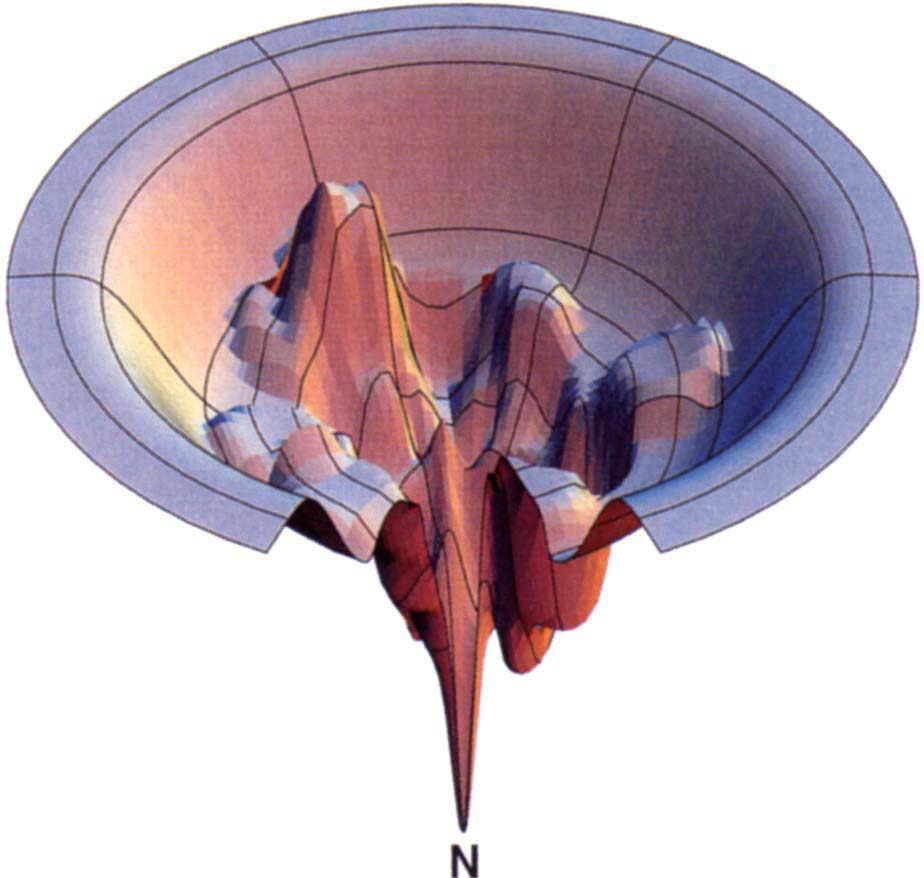
\includegraphics[width=2in]{figures/schematic/dill97-fig4}%
    \label{fig:folding:landscape}}
  \caption{\protect\subref{fig:folding:pathway} A ``double T'' example
    of the pathway model of protein folding, in which the protein
    proceeds from the native state $N$ to the unfolded state $U$ via a
    series of metastable transition states $I_1$ and $I_2$ with two
    ``dead end'' states $I_1^X$ and $I_2^X$.  Adapted from
    \citet{bedard08}.
    \protect\subref{fig:folding:landscape} The landscape model of
    protein folding, in which the protein diffuses through a
    multi-dimensional free energy landscape.  Separate folding
    attempts may take many distinct routes through this landscape on
    the way to the folded state.  Reproduced from
    \citet{dill97}.\label{fig:folding}}
  \end{center}
\end{figure}

When the choice of theoretical approach becomes murky, you must gather
experimental data to help distinguish between similar models.
Separating the pathway model from the funnel model is only marginally
within the realm of current experimental techniques, but with higher
throughput and increased automation it should be easier to make such
distinctions in the near future.


\section{Why \emph{single} molecule?}
\label{sec:single-molecule}

The large size of proteins relative to simpler molecules limits the
information attainable from bulk measurements, because the
macromolecules in a population can have diverse conformations and
behaviors.  Bulk measurements average over these differences,
producing excellent statistics for the mean, but making it difficult
to understand the variation.  The individualized, and sometimes rare,
behaviors of macromolecules can have important implications for their
functions inside the cell.  Single molecule techniques, in which the
macromolecules are studied one at a time, allow direct access to the
variation within the population without averaging.  This provides
important and complementary information about the functional
mechanisms of several biological systems\citep{bustamante08}.

Single molecule techniques provide an opportunity to study protein
folding and unfolding at the level of a single molecule, where the
distinction between the pathway model and funnel model is clearer.
They also provide a convenient benchmark for verifying molecular
dynamics simulations, because it takes lots of computing power to
simulate even one biopolymer with anything close to atomic resolution
over experimental time scales.  Even with significant computing
resources, comparing molecular dynamics results with experimental data
remains elusive.  For example, experimental pulling speeds are on the
order of \bareU{$\mu$m/s}, while simulation pulling speeds are on the
order of \bareU{m/s}\citep{lu98,lu99,rief02,zhao06,berkemeier11}.

% why AFM & what an AFM is
Single molecule techniques for manipulating biopolymers include
optical measurements, \ie, single molecule fluorescence microscopy and
spectroscopy, and mechanical manipulations of individual
macromolecules, \ie, force microscopy and spectroscopy using atomic
force microscopes (AFMs), laser tweezers\citep{kellermayer97,forde02},
magnetic tweezers\citep{smith92}, biomembrane force
probes\citep{merkel99}, and centrifugal
microscopes\citep{halvorsen09}.  These techniques cover a wide range
of approaches, and even when the basic approach is the same
(e.g.\ force microscopy), the different techniques span orders of
magnitude in the range of their controllable parameters.
%
\nomenclature[text ]{AFM}{Atomic force microscope (or microscopy).}

\section{Why \emph{un}folding?}
\label{sec:unfolding}

There's a lot of talk about protein \emph{folding} in this chapter,
while the rest of the thesis (and the title) are about
\emph{unfolding}.  If you understand protein folding, you can use your
understanding to design drugs with a particular conformation, or
predict the conformation of a biologically important receptor
(\cref{sec:folding-problem}).  Understanding protein unfolding is less
directly useful, because unfolded proteins are rarely biologically
relevant (although it does happen\citep{dyson05}).

The focus on unfolding is mainly because it's easier to unravel
proteins by pulling on their ends (\cref{sec:procedure}) than it is to
fold them into their native state by pushing on those ends
(\cref{fig:ligand-receptor,fig:I27}).  For proteins with smooth enough
energy landscapes, the folding and unfolding routes will be similar,
so knowledge about the unfolding behavior \emph{does} shed light on
the folding behavior.

Practically, the distinction between folding and unfolding makes
little difference, because drug designers and doctors are not
consuming SMFS results directly.  For researchers calibrating
molecular dynamics simulations, it doesn't matter if you compare
simulated folding experiments with experimental folding experiments,
or simulated unfolding experiments with experimental unfolding
experiments.  The important thing is to compare your simulation
against \emph{some} experimental benchmarks.  If your molecular
dynamics simulation successfully predicts a protein's unfolding
behavior, it makes me more confident that it will correctly predict
the protein's native folding behavior.


\section{Thesis outline}
\label{sec:outline}

\Cref{sec:methods} of this thesis outlines the apparatus and methods
for single molecule force spectroscopy with an atomic force
microscope.  \Cref{sec:sawsim} presents my \sawsim\ Monte Carlo
simulation for modeling unfolding/refolding behavior.  By comparing
model simulations with experimental measurements, we can gain insight
into the protein's kinetics.  After \cref{sec:sawsim}, you should have
a pretty firm grasp of the underlying physics, so we'll move on to
\cref{sec:pyafm} and discuss my \pyafm\ and \unfoldprotein\ experiment
control software.  With both the kinetic theory and procedure taken
care of, \cref{sec:calibcant} discusses thermal cantilever
calibration, deriving the theoretical approach and presenting my
\calibcant\ automatic calibration software.

Moving away from experiment control, \cref{sec:hooke} presents the
\Hooke\ suite for extracting unfolding force histograms (for
comparison with \sawsim\ simulations).  In \cref{sec:salt}, I pull all
the pieces together (experiment control, post processing, and
simulation) to carry out unfolding experiments on the
immunoglobulin-like domain 27 from human Titin (I27) in buffers with
different ionic strength.  We close with \cref{sec:future}, which
summarizes my conclusions and discusses possible directions for future
work.


\printnomenclature
% avoid index's second column overlapping the nomenclature space.
\iffinal{}{\pagebreak}
%\printindex

\begin{vita}

\begin{cv}{}

  \begin{cvlist}{Contact}
  \item W. Trevor King\\
    120 Miller St.\\
    Highlands, NJ, 07732
  \item Tel.:~(215)~284~6634\\
    Email:~wking@tremily.us
  \end{cvlist}

  \begin{cvlist}{Education}
  \item[09/2000--05/2004] Colgate University, Hamilton, NY
    (B.A.~in Physics and Math)

  \item[09/2004--05/2006] University of Rochester, Rochester, NY
    (M.A.~in Physics)

  \item[09/2006--05/2013] Drexel University, Philadelphia, PA
    (Ph.D.~track in Physics)
  \end{cvlist}

  \begin{cvlist}{Publications}
%    \begin{bibunit}[alpha]
%      \nocite{wking10}
%    \item[Books] \putbib
%    \end{bibunit}
    \item [Papers]
    \begin{bibunit}
      \nocite{
        king10}
      \putbib
    \end{bibunit}
    \item [Talks]
    \begin{bibunit}
      \nocite{
        2013-01-columbia,
        2009-10-life-cycles,
        2008-06-locks}
      \putbib
    \end{bibunit}
    \item [Posters]
    \begin{bibunit}
      \nocite{
        2013-04-swc,
        2011-04-saswsim,
        2010-04-open-source,
        2012-04-calibcant,
        2009-03-roughness,
        2008-04-sawsim,
        2008-02-stiffness}
      \putbib
    \end{bibunit}
  \end{cvlist}

  \begin{cvlist}{Teaching assistant-ships}
  \item[09/2004--05/2005] General Physics I
    (Mechanics)
  \item[Fall 2006] PHYS 152: Introductory Physics I
    (Mechanics)
  \item[Winter 2007] PHYS 101: Fundamentals of Physics I
    (Mechanics)
  \item[Spring 2007] PHYS 102: Fundamentals of Physics II
    (Electricity and magnetism)
  \item[Spring 2008] PHYS 102: Fundamentals of Physics II
    (Electricity and magnetism)
  \item[Fall 2008] PHYS 154: Introductory Physics III
    (Electricity, magnetism, and quantum mechanics)
  \item[Winter 2009] PHYS 201: Fundamentals of Physics III
    (Modern physics)
  \item[Summer 2009] PHYS 102: Fundamentals of Physics II
    (Electricity and magnetism)
  \item[Fall 2010] PHYS 405: Advanced Computational
    Physics---Parallel Computing
    (MPI and CUDA)
  \item[Winter 2011] PHYS 101: Fundamentals of Physics I
    (Mechanics)
  \item[Spring 2011] PHYS 102: Fundamentals of Physics II
    (Electricity and magnetism)
  \item[Fall 2011] PHYS 106: Introduction to Scientific Computing
    (Algorithms in Maple)
  \item[Winter 2012] PHYS 305: Computational Physics II
    (Algorithms in C and C++)
  \item[Spring 2012] PHYS 102: Fundamentals of Physics II
    (Electricity and magnetism)
  \item[Fall 2012] PHYS 405: Advanced Computational
    Physics---Parallel Computing
    (MPI and CUDA)
  \item[Winter 2013] PHYS 305: Computational Physics II
    (Algorithms in C and C++)
  \item[Spring 2013] PHYS 102: Fundamentals of Physics II
    (Electricity and magnetism)
  \end{cvlist}

  \begin{cvlist}{Research}
  \item[05/2002--09/2002] Vortex pinning in superconducting thin films.
    Wrote experimental control software in LabVIEW and fabricated
    samples using Nb sputtering, photolithography, and wet etching.
  \item[05/2003--09/2003] Navier--Stokes simulator.
    Ported a program simulating two dimensional incompressible
    fluid flow from MatLab to C.
  \item[09/2003--05/2004] Surface tension and lipid phase separation.
    Designed and began construction of an automated system for making
    rod pull equilibrium surface pressure measurements on phospholipid
    vesicle suspensions.  Completed drive chain hardware and LabVIEW
    software for sequentially moving samples to the rod pull mechanism
    for measurement.
  \item[05/2005--05/2006] Superconducting phase qubit quantum computing.
    Wrote experiment control software in LabVIEW and data analysis
    software in MatLab.  Managed the $^3$He dilution refrigerator and
    assembled custom circuit boards.
  \item[09/2006--07/2013] Single molecule force spectroscopy via AFM.
    Designed calibration, experiment control, data processing, and
    Monte Carlo simulation software in Python and C.  Performed
    necessary hardware troubleshooting and maintenance.
  \end{cvlist}

  \begin{cvlist}{System administration}
  \item[09/2009--09/2011] Drexel physics department webmaster.
    Maintained and streamlined department website and assisted with
    Apache-to-SiteCore migration.
  \item[09/2005--Present] Home newtork system adminstrator.
    I run Linux systems (primarily Gentoo) at home.  I use my home
    network to test installation, deployment, and maintenance of the
    software infrastructure I'd like to see at work, which has lead to
    experience with many packages (highlights below).  Since 2008 I've
    been publishing my notes on these systems in my blog at
    \url{http://blog.tremily.us/}.
  \end{cvlist}

  \begin{cvlist}{Software}
  \item[Operating systems]
    \href{http://www.gentoo.org/}{Linux (Gentoo)}
  \item[Languages]
    \href{http://python.org/}{Python},
    \href{http://en.wikipedia.org/wiki/C_\%28programming_language\%29}{C},
    \href{http://tiswww.case.edu/php/chet/bash/bashtop.html}{Bash},
    \href{http://www.w3.org/html/wg/drafts/html/master/}{HTML},
    \href{http://www.w3.org/XML/}{XML},
    \href{http://www.w3.org/Style/CSS/Overview.en.html}{CSS},
    \href{http://www.sqlite.org/}{SQLite},
    \href{https://www.djangoproject.com/}{Django},
    \href{http://en.wikipedia.org/wiki/JavaScript}{JavaScript},
    \href{http://www.ni.com/labview/}{LabVIEW},
    \href{http://us.php.net/}{PHP}
  \item[Creator]
    \href{https://pypi.python.org/pypi/pygrader}{pygrader},
    \href{https://pypi.python.org/pypi/pyassuan}{pyassuan},
    \href{https://pypi.python.org/pypi/pgp-mime}{pgp-mime},
    \href{https://pypi.python.org/pypi/quizzer}{quizzer},
    \href{http://blog.tremily.us/posts/sawsim/}{sawsim},
    \href{https://pypi.python.org/pypi/pycomedi}{pycomedi},
    \href{https://pypi.python.org/pypi/pypiezo}{pypiezo},
    \href{https://pypi.python.org/pypi/stepper}{stepper},
    \href{https://pypi.python.org/pypi/pypid}{pypid},
    \href{https://pypi.python.org/pypi/pyafm}{pyafm},
    \href{https://pypi.python.org/pypi/calibcant}{calibcant},
    \href{https://pypi.python.org/pypi/stepper}{unfold-protein},
    \href{https://pypi.python.org/pypi/chemdb}{chemdb},
    \href{https://pypi.python.org/pypi/igor}{igor},
    \href{https://pypi.python.org/pypi/h5config}{h5config},
    \href{https://pypi.python.org/pypi/FFT-tools}{FFT-tools},
    \href{https://pypi.python.org/pypi/update-copyright}{update-copyright},
    \href{https://pypi.python.org/pypi/mutt-ldap}{mutt-ldap},
    \href{http://blog.tremily.us/posts/Course_website/}{course-website},
    \href{http://blog.tremily.us/posts/problempack/}{problempack},
    \href{http://git.tremily.us/?p=assignment-template.git}{assignment-template},
    \href{http://blog.tremily.us/posts/Gentoo_overlay/}{wtk-overlay},
    \href{https://github.com/wking/dotfiles-framework}{dotfiles-framework}
  \item[Maintainer]
    \href{http://github.com/wking/rss2email/}{rss2email},
    \href{http://bugseverywhere.org/}{Bugs Everywhere},
    \href{http://blog.tremily.us/posts/drexel-thesis/}{drexel-thesis},
    \href{https://pypi.python.org/pypi/Hooke/}{Hooke}
  \item[Contributor]
    \href{http://software-carpentry.org/}{Software Carpentry},
    \href{http://git-scm.com/}{Git},
    \href{http://docs.getpelican.com/}{Pelican},
    \href{http://www.gentoo.org/proj/en/releng/catalyst/}{Gentoo catalyst},
    \href{https://github.com/agrover/python-kmod}{python-kmod},
    \href{http://www.comedi.org/}{Comedilib},
    \href{http://web.mit.edu/kerberos/}{Kerberos},
    \href{http://www.kernel.org/}{Linux kernel},
    \href{http://www.cython.org/}{Cython},
    \href{http://ikiwiki.info/}{ikiwiki},
    \href{http://www.gnuplot.info/}{gnuplot},
    \href{https://github.com/wking}{and}
    \href{http://www.ohloh.net/accounts/wking}{more}
    \href{http://blog.tremily.us/posts/Bugs/}{\ldots}
  \item[User]
    \href{http://www.gnu.org/software/emacs/}{Emacs},
    \href{http://www.latex-project.org/}{\LaTeX},
    \href{http://nginx.org/}{Nginx},
    \href{http://www.openldap.org/}{OpenLDAP},
    \href{http://www.postfix.org/}{Postfix},
    \href{https://www.isc.org/software/bind}{BIND},
    \href{http://www.cups.org/}{CUPS},
    \href{http://www.openssh.org/}{OpenSSH}
    \href{http://en.wikipedia.org/wiki/Network_File_System#NFSv4}{kerberized
      NFSv4},
    \href{http://mlmmj.org/}{mlmmj}
  \end{cvlist}

%  \cvplace{Highlands, NJ}
%  \date{\today}
  \date{}
\end{cv}

\end{vita}


\end{document}
